%% -*- coding:utf-8 -*-
%%%%%%%%%%%%%%%%%%%%%%%%%%%%%%%%%%%%%%%%%%%%%%%%%%%%%%%%%
%%   $RCSfile: hpsg-partikel.tex,v $
%%  $Revision: 1.18 $
%%      $Date: 2008/09/30 09:14:41 $
%%     Author: Stefan Mueller (CL Uni-Bremen)
%%    Purpose: 
%%   Language: LaTeX
%%%%%%%%%%%%%%%%%%%%%%%%%%%%%%%%%%%%%%%%%%%%%%%%%%%%%%%%%
\newcommand{\anf}{\emph{an$_5$}\xspace}%
\newcommand{\los}{\emph{los}\xspace}


\chapter{Partikelverben}
\label{chap-partikel}

In\is{Verb!Partikel-|(} diesem Kapitel werden die Partikelverben besprochen. Diese sind
aus syntaktischer und auch aus morphologischer Sicht interessant,
und es wurde oft versucht, die Partikelverben entsprechend der Vorlieben
des jeweiligen Forschers der Morphologie oder der Syntax allein zuzuschlagen.
Wie die Diskussion in diesem und im folgenden Kapitel zeigen wird, ist
es sinnvoller, Partikelverben sowohl in der Syntax als auch in der Morphologie
zu behandeln. In diesem Kapitel werden die syntaktischen Eigenschaften
von Partikelverben diskutiert, und es wird eine entsprechende Analyse vorgestellt.
Im folgenden Kapitel wird erklärt, wie die morphologischen Eigenschaften
von Partikelverben modelliert werden können.

Die in diesem und im folgenden Kapitel entwickelte Analyse der Partikelverben stellt
den Höhepunkt des Buches dar: Die Analysen aus vorangegangenen Kapiteln interagieren
bei der Analyse der Partikelverben. Wir benötigen Adjunktion (Kapitel~\ref{chap-adjunkte}),
Lexikonregeln (Kapitel~\ref{chap-lexikon}), die Verbstellung und Konstituentenstellung 
(Kapitel~\ref{chap-Konstituentenreihenfolge}), Vorfeldbesetzung (Kapitel~\ref{chap-nla}),
Kasuszuweisung (Kapitel~\ref{chap-kasus}),
Argumentanziehung (Kapitel~\ref{chap-verbalkomplex}) und Passiv (Kapitel~\ref{chap-passiv}).

\section{Das Phänomen}

Im Deutschen gibt es eine Klasse von Verben, die durch
morphologisches Material (\mex{1}) oder syntaktisches
Material (\mex{2}) in zwei Teile geteilt werden können. 
Der Teil, der bei Verbletztstellung links vom Verb steht und
der zurückbleibt, wenn das Verb vorangestellt wird, wird
traditionell \emph{abtrennbares Präfix}\is{Pr"afix!abtrennbares} genannt. Da Präfixe
so definiert sind, dass sie nicht abtrennbar sind, verwenden
die meisten Wissenschaftler heute die Bezeichnung \emph{Verbpartikel}\is{Verbpartikel}.
Andere Bezeichnungen sind \emph{Verbzusatz}\is{Verbzusatz} und \emph{Präverb}\is{Pr"averb} \citep[\page99]{Jung67a}.
%%         \citet[\page10]{Stiebels96a} benutzt \emph{Verbzusatz} aber, um
%%         sowohl auf Partikel als auch auf Präfixe zu referieren.
%%         \citet{Fourquet74a} benutzt the term
%%         particle both for prefixes and for particles that can be separated from
%%         their verb. 
%% %Steinitz69a:37 trennbares Verbalpräfix
%% % wohl auch Zifonun73a
%% \citet{Luedeling98a} uses the term preverb\is{preverb}
%%         in a sense that also includes ordinary adverbs.%
%% %
%% %        In what follows, I stick to the terminology introduced above.
%}
In (\mex{1}) sind die Partikel \emph{über} und der Stamm des Basisverbs (\stem{setz})
durch das \emph{ge}"=Präfix bzw.\ durch den Infinitivmarkierer \emph{zu} voneinander getrennt.
\eal
\ex\iw{übersetzen}
Der Fährmann hat Karl übergesetzt.
\ex
Der Fährmann versucht, Karl überzusetzen.
\zl
In (\mex{1}a,b) befindet sich das Verb in der linken Satzklammer und die Partikel bleibt zurück.
\eal
\ex
Setzt der Fährmann Karl über?
\ex
Der Fährmann setzt Karl über.
\label{ex-setzt-ueber}
\ex
dass der Fährmann Karl übersetzt
\zl
Die Partikel wird rechts von allen nicht"=extraponierten Argumenten und Adjunkten
angeordnet. Die Partikel bildet die rechte Satzklammer. Hierin unterscheiden sich Partikelverben
von Präfixverben. Die Präfixverben werden nicht aufgeteilt, wenn das Verb in Initialstellung
steht:
\eal
\ex Der Fährmann übersetzt das Buch.
\ex Der Fährmann setzt das Buch über.
\zl
(\mex{0}) kann nur bedeuten, dass der Fährmann das Buch in eine andere Sprache überträgt.
In (\mex{0}b) entsteht ein komischer Effekt, weil das Verb nur in der Lesart \emph{Gewässer überqueren}
verstanden werden kann und weil in dieser Lesart das Objekt normalerweise -- sieht man mal von Kohlköpfen ab --
belebt ist.

Viele Partikeln entsprechen Adjektiven\is{Adjektiv} (\mex{1}a), Adverbien\is{Adverb} (\mex{1}b), Nomen\is{Nomen} (\mex{1}c), 
Präpositionen\is{Pr"aposition} (\mex{1}d) oder Verben\is{Verb} (\mex{1}e).
\eal
\ex\iw{trockenlegen}
Sie legten die Sümpfe trocken.
\ex\iw{weglaufen}
Er lief weg.
\ex\iw{Rad fahren}
Er fuhr Rad.
\ex\iw{umfärben}
Er färbte den Mantel um.
\ex\iw{sitzenbleiben}
Er blieb sitzen.
\zl
%
Es gibt aber auch Partikeln wie \emph{dar} (\word{darlegen}), 
\emph{inne} (\word{innehalten}) und \emph{acht} 
(\word{achtgeben}), die nicht unter diese Kategorien fallen.
Außerdem gibt es Partikelverben, zu denen es kein entsprechendes Basisverb ohne
Partikel gibt. Beispiele sind \word{abstatten} in \emph{einen Besuch abstatten} und 
\word{anstrengen} in \emph{sich anstrengen}. Partikelverben können
auch ein Basisverb enthalten, das von einem Adjektiv (\mex{1}a) oder einem Nomen (\mex{1}b) abgeleitet ist.\footnote{
        \citew*[\page20]{SW92}.%
}
\eal
\ex auf"|heitern, auf"|hellen
\ex ein"-ölen, eindellen, ankreuzen, anprangern
\zl

\subsection{Transparente und nicht"=transparente Partikelverben}

Man unterscheidet zwischen transparenten und nicht"=transparenten Partikelverben. Wörter
sind nicht"=transparent, wenn man im heutigen Deutsch nicht erklären kann, wie sich die
Gesamtbedeutung eines Wortes aus der Bedeutung seiner Bestandteile ergibt. \emph{anfangen}
ist \zb ein nicht"=transparentes Partikelverb, da die Bedeutung, die das Verb \emph{fangen}
hat, im Partikelverb nicht wiederzufinden ist. Auf der anderen Seite gibt es viele transparente
Partikelverbbildungen und auch Kombinationsmuster, die produktiv sind. Was die Sache
für diejenigen, die anfangen, sich mit Partikelverben zu beschäftigen, unübersichtlich macht, ist,
dass eine Verbpartikel durchaus verschiedene Bedeutungen haben kann und somit
neben eventuellen nicht"=transparenten Mustern auch in verschiedenen
produktiven oder nicht"=produktiven transparenten Mustern vorkommen kann.
\citet{Stiebels96a} hat die Partikeln \emph{an} und \emph{auf} systematisch untersucht.
Für \emph{an} schlägt sie neben einem \emph{an} für idiomatische Partikelverben wie \emph{anfangen}
die folgenden sechs Varianten vor:

\eal
\label{verschiedene-ans}
\ex an$_1$: anheften, ankleben, annähen                           \jambox*{\citep[Kapitel~6.1.2]{Stiebels96a}}
\ex an$_2$: anjagen,  anhüpfen, anschleichen, anrennen            \jambox{\citep[Kapitel~6.1.2]{Stiebels96a}}
\ex an$_3$: anerziehen, antrainieren                              \jambox{\citep[Kapitel~7.1.2]{Stiebels96a}}
\ex an$_4$: anmachen, anknipsen, anschalten                       \jambox{\citep[Kapitel~7.3.5]{Stiebels96a}}
\ex an$_5$: angrapschen, anpacken, anrühren, antatschen, antippen,
            anfahren, anfliegen, anfunken, anspielen              \jambox{\citep[Kapitel~7.4.1]{Stiebels96a}}
\ex an$_6$: anschmoren, anlesen, anspielen                        \jambox{\citep[Kapitel~5.2.3]{Stiebels96a}}
\zl
(\mex{0}a) wird mit kausativen Kontaktverben, Verben des Befestigens gebildet. In
(\mex{0}b)
%% \NOTE{JB: Es wird nicht ganz klar, wozu die Unterscheidungen gebraucht werden. (Außer bei
%% produktiv/unproduktiv) Semantik?}
werden Bewegungsverben mit \emph{an} kombiniert. Das Muster in (\mex{0}c) mit Wissensübertragungsverben
ist nach \citet[\page 130]{Stiebels96a} nicht produktiv, obwohl sich neue Formen über Analogie bilden lassen.
In (\mex{0}d) entspricht das \emph{an} einem prädikativen \emph{an}, wie es in (\mex{1}) vorkommt:
\ea
Die Lampe ist an.
\z
Für die Kombination mit \emph{an$_5$} kommen nach Stiebels agentive intransitive Verben in Frage,
und das Muster ist hochgradig produktiv.
\emph{an$_6$} ist ebenfalls produktiv. Durch diese Partikel wird angezeigt, dass die vom Basisverb
bezeichnete Handlung bis zu einem gewissen Grad jedoch nicht vollständig ausgeführt
wird. \emph{an$_6$} kann nur mit Verben kombiniert werden, die inkrementelle oder dekrementelle
Prozesse beschreiben, so dass ein vorzeitiger Abbruch plausibel ist.


Betrachtet man Partikelverben wie \emph{anfangen}, so scheint es gerechtfertigt, Partikelverben einfach
ins Lexikon zu schreiben. Würde man alle Partikelverben ins Lexikon schreiben, würde man aber der Tatsache
nicht gerecht, dass es produktive Muster gibt, \dash Muster, die auch auf neu entstandene Verben anwendbar
sind. Für solche Fälle muss man Regeln finden, die die Regelmäßigkeiten erfassen. In der HPSG liegt
es nahe, dafür Lexikonregeln zu verwenden. In diesem Kapitel werden solche Lexikonregeln formuliert,
wir beschäftigen uns außerdem mit den syntaktischen Eigenschaften der Partikelverben.
Ich werde in den folgenden Abschnitten zeigen, dass Partikel und Verb sich wie Verben verhalten,
die einen Komplex bilden. Das heißt, dass man die Analyse, die im Kapitel~\ref{chap-verbalkomplex}
für den Verbalkomplex entwickelt wurde, für Partikelverben übernehmen kann.

\subsection{Konstituentenstellung}
\label{sec-linearization}%
\label{sec-partlinearization}
%\is{serialization|(}
\label{sec-linearization-pv-mf}


Die Partikel \emph{an} kann mit intransitiven Verben
wie \emph{lachen} in (\mex{1}a) kombiniert werden. Das Resultat ist ein transitives Verb (\mex{1}c).
Die von der Partikel eingeführten Argumente (wie \zb \emph{ihn} in (\mex{1}c)) können frei
mit den Argumenten des Basisverbs vertauscht werden, wie (\mex{1}d) zeigt:
\eal
\label{ex-anlachen-perm-mf}
\ex[]{
dass niemand lacht.
}
\ex[*]{
dass niemand ihn lacht
}
\ex[]{\iw{anlachen}
dass    niemand      ihn anlacht
}
\ex[]{\iw{anlachen}
dass    ihn       niemand      anlacht
}
\zl
Das ist parallel zu den kohärenten Konstruktionen, die im Kapitel~\ref{chap-verbalkomplex}
bzw.~\ref{chap-anhebung} diskutiert wurden. Als Beispiel für eine solche kohärente Konstruktion
sei hier die Einbettung von \emph{lachen} unter das AcI"=Verb \emph{sehen} angegeben:
\eal
\ex dass niemand ihn lachen sieht
\ex dass ihn niemand lachen sieht
\zl


\subsubsection{Verbstellung}

Wenn man annimmt, dass die Verbindung von Partikel und Verb parallel zur Verbalkomplexbildung 
ist, ist auch sofort erklärt, warum das Verb ohne die Partikel vorangestellt werden kann. Die Voranstellung
in (\mex{1}) ist dann parallel zu der in (\mex{2}):
\eal
\ex weil er ihn anlacht
\ex Lacht er ihn an?
\zl

\eal
\ex weil er ihn lachen sieht
\ex Sieht er ihn lachen?
\zl

\noindent
Es ist auch klar, warum nicht das gesamte Partikelverb vorangestellt werden kann,
denn in Verbalkomplexen wird auch immer nur das Finitum, also das maximal übergeordnete
Element vorangestellt. (\mex{1}a) ist also aus demselben Grund ungrammatisch wie (\mex{1}b):
\eal
\ex[*]{
Er [anlacht] ihn.
}
\ex[*]{
Er [schlafen sieht] ihn.
}
\zl

\subsubsection{Vorfeldbesetzung}
\label{sec-part-vorfeldbesetzung}

Auch\is{Extraktion|(}\is{Vorfeldbesetzung|(} die Vorfeldbesetzungen ähneln denen, die bei Verbalkomplexen
möglich sind. Es wird zwar oft behauptet, dass die Partikel nicht ins Vorfeld gestellt werden kann,\footnote{
  Diese Behauptung findet man in verschiedenen Versionen in der Literatur. Zu einer
  ausführlichen Diskussion der Behauptungen siehe \citew{Mueller2002b,Mueller2002d}.%
} dies ist jedoch nicht korrekt, wie die folgenden Belege zeigen:\footnote{
Bei (\ref{aus-dem-schema-aus-bricht}) handelt es sich um ein Beispiel, in dem
die Partikel durch eine vollständige Präpositionalphrase spezifiziert wird \citep{Olsen97a,Olsen99a}.
Weitere Beispiele hierfür sind:
\eal
\ex Er legte die Folie auf den Projektor auf.
\ex Er warf die Briefe in den Briefkasten ein.
\zl 
(\ref{aus-dem-schema-aus-bricht}) zeigt, dass die vollständige PP gemeinsam mit der Partikel voranstellbar ist.%
}

\eal
\label{bsp-partikel-fronting}
%\ex \emph{Los}  \emph{ging} es schon   in dieser Woche. (taz, 11.10.95, S.\,4)
\ex \emph{Los} \emph{geht} es diesen Mittwoch, [\ldots], mit einem einführenden Vortrag\footnote{
  Anatol Stefanowitsch, talks@cl.uni-bremen.de, 26.04.2004.
}
\ex
\label{bsp-vor-hat-er-das}
\emph{Vor} \emph{hat} er das jedenfalls.\footnote{
taz, 15.07.1999, S.\,19.
}
\ex \emph{Entgegen} \emph{kam} der EuGH den Streitkräften, indem er \ldots{}\footnote{
taz, 12.01.2000, S.\,1.}
\ex Es klopfte, \emph{eintrat} der Studienrat.\footnote{
Walser, \emph{Ohne einander}, S.\,51, zitiert nach \citew*[\page1621]{Hoberg97a}.
}
\ex\label{bsp-auf-faellt}
\emph{Auf}  \emph{fällt}, da"s \ldots{}\footnote{
  \citew[\page62]{Duden-rs-91}.
}
\ex\label{bsp-auf-wachte}
Nach einigen Zügen, "`die irgendwie komisch schmeckten"', fielen dem Interviewten die Augen zu. 
\emph{Auf wachte} der "`39jährige Mitarbeiter des Mitropa-Fahrbetriebes, Mitglied der SED. Glücklich verheiratet, drei Kinder"'
erst % im     stand das `im' im Text, oder habe ich das reingetypot
wieder im Westen [\ldots] -- gerade rechtzeitig, um "`einen Packen D-Mark-Scheine auf dem Tisch"' 
des "`gewissenlosen Schleppers"' zu sehen.\footnote{
  Die Menthol-Affäre, taz, 03.11.2004, S.\,17.
}
\ex \emph{Fehl} \emph{schlug} auch der Versuch, über die örtliche Kinderärztin die Identität des Mädchens zu erfahren.\footnote{
  Frankfurter Rundschau, 30.08.1997, S.\,22.
}
\ex\label{aus-dem-schema-aus-bricht}
{}[\ldots] dass der Unterschied zwischen den beiden sich über die Jahre kaum verändert hat: [\ldots]
    \emph{Aus dem Schema aus} \emph{bricht} lediglich das Jahr 2003.\footnote{
    taz, 22.07.2005, S.\,19.
}
\zl
Zu weiteren Daten siehe \citew{Mueller2002b,Mueller2002d}.


Interessanterweise können jedoch infinite Verben nicht ohne die Partikel vorangestellt werden.\footnote{
        Siehe \citew[\page101]{Hoehle82b}, \citew[\page721]{Haftka81a}, \citew*[\page127]{Olszok83}, % FVG
        \citew[\page212]{Loetscher85a} und \citew*[\page104]{Uszkoreit87a} zu ähnlichen Beispielen.
%        Lötscher explicitly discusses the similarity to verbal complexes.
}
In (\mex{1}) sind entsprechende Beispiele zu sehen:
\eal
\label{ex-fronting-part-stranded}
\ex[*]{
Fahren wird Karl Bus / Rad.
}
\ex[*]{
Stehen werden sie  Schlange.
}
\ex[*]{
Kommen wird er frei.
}
\ex[*]{\label{bsp-kommen-wird-karl-an}
Kommen wird Karl an.
}
\ex[*]{
Schlafen wird Karl ein.
}
\ex[*]{
Fangen will Karl das Buch zu lesen an.
}
\zl

\noindent
Die Beispiele für Partikelvoranstellung in (\ref{bsp-partikel-fronting}) ähneln Verbvoranstellungen wie denen in (\mex{1}).
\eal
\ex Lachen wird er müssen.
\ex Singen wird er das Lied.
\zl
Die Verbvoranstellung wurde im Kapitel~\ref{sec-pvp} besprochen. (\mex{0}b) zeigt,
dass das Verb \emph{singen} ohne seine Argumente vorangestellt werden kann.
Dass bei entsprechender Kontrastierung auch die Voranstellung einer Partikel,
die Argumente beisteuert, möglich ist, zeigt (\ref{bsp-an-hat-er-ihn-nicht-gelacht}):
\ea
\label{bsp-an-hat-er-ihn-nicht-gelacht}
An hat er ihn nicht gelacht, sondern aus.
\z

\noindent
Die ungrammatischen Beispiele in (\ref{ex-fronting-part-stranded}) sind
parallel zu dem Beispiel in (\mex{1}), das ebenfalls im Kapitel~\ref{sec-pvp}
diskutiert wurde.
\ea[*]{
\label{ex-pvp-ungram-zwei}
Müssen wird er ihr ein Märchen erzählen.
}\label{ex-muessen-wird-er-ihr-zwei}
\z
Die Generalisierung in bezug auf diese Daten ist, dass Teile des Prädikatskomplexes
nur vorangestellt werden können, wenn alle Prädikatskomplexteile, die vom vorangestellten
Material regiert werden, ebenfalls vorangestellt werden.
So regiert \zb \emph{müssen} in (\mex{0}) \emph{erzählen}.
Wenn \emph{müssen} vorangestellt wird, muss \emph{erzählen} ebenfalls vorangestellt werden.

Überträgt man diese Analyse auf Partikelverben, ist erklärt, warum \zb \emph{ankommen}
nicht wie in (\ref{bsp-kommen-wird-karl-an}) aufgespalten werden kann:\footnote{
  Siehe auch \citew*{Hoehle82b} für einen Vorschlag, für die
  Kombination von Partikel und Verb dieselbe Regel wie für den Verbalkomplex zu benutzen.%
}
Da \emph{an} und \emph{kommen}
Bestandteil des Prädikatskomplexes sind und da \emph{kommen} die Partikel \emph{an} regiert,
muss diese mit ins Vorfeld, wenn \emph{kommen} vorangestellt wird:
\ea
Ankommen wird Karl.
\z
\is{Extraktion|)}\is{Vorfeldbesetzung|)}



\section{Die Analyse}
\label{sec-pv-anal}

In den folgenden Abschnitten zeige ich, wie ein Lexikoneintrag
für ein nicht"=transparentes Partikelverb aussieht und stelle
eine Lexikonregel vor, die Verbeinträge lizenziert, die mit verschiedenen
Partikeln in produktiv auf"|tretenden Mustern verwendet werden können.
Analysen für die Verbstellung und die Voranstellung der Partikel
werden ebenfalls vorgestellt.

\subsection{Lexikoneinträge für nicht"=transparente Partikelverben und die Analyse der Verbstellung}
\label{le-nontr-part-verb}

Die Struktur in (\mex{1}) zeigt den \locw des Lexikoneintrags für das
nicht"=transparente Partikelverb \emph{vorhaben}.\NOTE{Rollen von \emph{vorhaben}???}
%
\eas
(\emph{vor}) \emph{hab-} (nicht-transparentes Partikelverb):\label{le-vorhaben}
\\
\ms{
cat & \ms{
%       head   & verb\\
       comps & \liste{ NP[\type{str}]\ind{1}, NP[\type{str}]\ind{2}, Part[\type{vor}, lex+] } \\
                                     } \\
cont & \ms[vorhaben]{
                                        arg1 & \ibox{1} \\
                                        arg2 & \ibox{2} \\
                                    } \\
}
\zs

\noindent
Der semantische Beitrag des Partikelverbs wird nicht kompositional aus der Bedeutung
des Verbs und der Partikel ermittelt, wenn diese im Satz kombiniert werden, sondern
ist bereits im \contw des Stammeintrags repräsentiert. Die Form der Partikel,
die mit einer flektierten Form des Stammes kombiniert werden muss, wird in der
\compsl genau angegeben.

%% I follow \citet[\page 238]{Olsen99c} and 
%% \citet[\page 44]{McIntyre2001a} in assuming that
%% particles like \emph{vor} are not prepositions, but are related to prepositions by
%% lexical redundancy rules. Hence, the element in \xcomp is not of category P or PP, but \textsc{Part}.
Abbildung~\vref{fig-Aicke-das-vor-hat} zeigt die Analyse für das Beispiel (\mex{1}), in dem
das Verb in Letztstellung steht.
\ea
weil    Aicke das  vorhat
\z
\begin{figure}
\begin{forest}
sm edges
[{V[\textsc{comps} \eliste]}
   [{\ibox{1} NP[\type{nom}]} [Aicke]] 
   [{V[\textsc{comps} \sliste{ \ibox{1} }]}
     [{\ibox{2} NP[\type{acc}]} [das]] 
   [{V[\textsc{comps} \sliste{ \ibox{1}, \ibox{2} }]}
     [\ibox{3} Part [vor]]
     [{V[\textsc{comps} \sliste{ \ibox{1}, \ibox{2}, \ibox{3} }]} [hat]]]]]
\end{forest}
\caption{\label{fig-Aicke-das-vor-hat}Analyse von \emph{weil Aicke das vorhat}}
\end{figure}
Dabei wird \emph{vor} mit \emph{hat} mit dem Prädikatskomplexschema (siehe Seite~\pageref{schema-vk}) kombiniert.

Da \emph{vorhat} finit ist, wird das Subjekt als Element der \compsl repräsentiert.
Partikel und Verb werden in einer Struktur vom Typ \type{head-cluster-phrase} kombiniert.
Das Akkusativobjekt und das Subjekt werden durch das Kopf"=Argument"=Schema lizenziert.
Da das Kopf"=Argument"=Schema die Sättigung von Argumenten in beliebiger Reihenfolge zuläßt,
können die beiden Abfolgen von Subjekt und Objekt in (\mex{1}) erklärt werden.
\eal
\ex weil das niemand vorhat
\ex weil niemand das vorhat
\zl
Da die Partikel \lex\isfeat{lex} + sein muss, kann das Kopf"=Argument"=Schema nicht benutzt werden, um
Anordnungen abzuleiten, bei denen die Partikel im Mittelfeld steht. Für solche Abfolgen gibt es zwar
Belege \citep[\page 50]{Luedeling2001a}, bei entsprechenden Umstellungen gibt es aber spezielle informationsstrukturelle Effekte, so
dass diese Strukturen anders als normale Umstellungen im Mittelfeld zu analysieren sind.


Für den Satz in (\mex{1}), in dem das Verb in Initialstellung steht, nehme ich die Analyse in 
Abbildung~\vref{fig-hat-er-das-vor} an.
\ea
Hat Aicke das vor?
\z
\begin{figure}
\begin{forest}
sm edges
[{V[\textsc{comps} \sliste{ }]}
   [{V[\textsc{comps} \sliste{ \ibox{4} }]}
     [{V[\textsc{comps} \sliste{ \ibox{1}, \ibox{2}, \ibox{3} }]} [hat]]]
     [{\ibox{4} V[\textsc{comps} \eliste]}
       [{\ibox{1} NP[\type{nom}]} [Aicke]]
       [{V[\textsc{comps} \sliste{ \ibox{1} }]}
          [{\ibox{2} NP[\type{acc}]} [das]]
          [{V[\textsc{comps} \sliste{ \ibox{1}, \ibox{2} }]}
            [\ibox{3} Part [vor]]
            [{V[\textsc{comps} \sliste{ \ibox{1}, \ibox{2}, \ibox{3} }]} [\trace]]]]]]
\end{forest}
\caption{\label{fig-hat-er-das-vor}Analyse von \emph{Hat er das vor?}}
\end{figure}
Diese Analyse ist die ganz normale Verbbewegungsanalyse, die in Kapitel~\ref{sec-v1}
vorgestellt wurde: Die Lexikonregel für die Verberststellung wird auf einen Eintrag angewendet,
der die Verbpartikel selegiert. Die Information über die Valenz des Eingabeverbs der
Lexikonregel wird über DSL zur Verbspur transportiert, und da sie dort mit der
Valenzinformation der Spur identifiziert wird, verhält sich die Spur genau so,
als stünde an ihrer Stelle das Eingabeverb. Die Spur bildet mit der Partikel einen
Komplex, so wie das in Abbildung~\ref{fig-Aicke-das-vor-hat} für Verb und Partikel der
Fall ist.

Nach dieser Diskussion der Repräsentation nicht"=transparenter Partikelverben und 
der grundlegenden Eigenschaften der Kombination von Partikel und Verb, möchte ich
im folgenden Partikelverbkombinationen erklären, die einem produktivem Muster folgen.



\subsection{Lexikoneinträge für produktive Partikelverbkombinationen}
\label{sec-lr-for-transp-pvs}


Eine große Gruppe von Partikelverben ist transparent und kann kompositional analysiert
werden. Im folgenden werde ich Beispielanalysen für transparente Partikelverben geben,
die für bestimmte Partikelverbklassen stehen. Ich diskutiere Partikelverben mit \emph{los},
wie \zb \emph{loslachen} und Partikelverben mit Stiebels' \emph{an$_5$}, wie \zb \emph{anlachen}.
Das \emph{los} ist ein Aspektmarker,\is{Aspekt} der nichts zur Valenz des Partikelverbs beisteuert.
Das zeigen die Beispiele in (\mex{1}):
\eal
\ex[]{\iw{lachen}
Er lacht.
}
\ex[]{\label{ex-loslacht}\iw{loslachen}\iw{los}
Er lacht los.
}
\ex[*]{
Er lacht sie los.
}
\zl
(\mex{0}c) zeigt, dass es nicht möglich ist, ein zusätzliches nicht vom Verb
selegiertes Argument zu haben.\footnote{
  Es gibt eine Lesart, in der das \emph{los} so viel wie \emph{ab} oder \emph{frei}
  bedeutet, diese ist jedoch hier nicht von Interesse,
  da es sich -- wenn diese Lesart vorliegt -- um eine andere Konstruktion,
  nämlich um eine Resultativkonstruktion\is{Resultativkonstruktion}, handelt
  (siehe \citew[\page381]{Mueller2002b}).%
}
Die Sätze in (\mex{1}a,b) zeigen, dass transitive Verben nicht mit der Partikel \emph{los}
kombiniert werden können, wenn das Objekt ausgedrückt wird:
\eal
\ex[*]{\iw{loslesen}
Er liest das Buch los.
}
\ex[]{
Er liest los.
}
\zl
Im Unterschied zu \emph{los} lizenziert \anf ein zusätzliches Argument:
\eal
\ex[]{\label{ex-anlachen}\iw{anlachen}
Er lacht  sie an.
}
\ex[*]{
Er lacht sie.
}
\zl
Das Basisverb muss intransitiv and agentiv
sein \citep[\page950]{SW94a}. Der Unterschied zwischen \emph{los} und \anf legt nahe,
dass die jeweilige Partikel für die Argumentstruktur des gesamten Partikelverbs
mitverantwortlich ist: \anf lizenziert ein zusätzliches Argument, \los dagegen nicht.
Beide Partikeln können nur mit intransitiven bzw.\ ohne Objekt verwendeten Verben
kombiniert werden.

Die Partikeln passen nicht zu beliebigen Verben. Die semantische Klasse
des Basisverbs wird von der Partikel vorgegeben. Es wäre nicht korrekt, die Partikel
als Kopf zu analysieren, wie das \zb von \citet[\page 438]{Trost91a} vorgeschlagen wurde, 
da die Rektionsverhältnisse im Verbalkomplex adäquater
mit dem Verb als Kopf erfaßt werden können. Ich schlage deshalb vor,
Partikeln wie \emph{los} und \anf als Modifikatoren\is{Modifikator} zu analysieren. Den Lexikoneintrag
für \emph{los} zeigt (\mex{1}):

\eas
\label{le-los-asp}
\mbox{\emph{los} (Aspektmarker):}\\
\ms{
cat & \ms{ head & \ms[particle]{ mod  & \textrm{V[\textsc{comps} \sliste{ NP[\str] }, \textsc{cont} \ibox{1}]} \\
                                 subj & \eliste \\
                               } \\
           comps & \eliste \\
         }\\
cont & \ms[beginnen]{ soa & \ibox{1} \\
                 } \\
}
\zs\iw{los|uu}
Die Adjunktanalyse, die in Kapitel~\ref{chap-adjunkte} vorgestellt wurde,
geht davon aus, dass Adjunkte den Kopf, den sie modifizieren, über das \modm selegieren.
Da der Wert von \textsc{mod} ein \type{synsem}"=Objekt ist, können sowohl syntaktische als auch semantische
Eigenschaften des modifizierten Kopfes selegiert werden. Im Lexikoneintrag für \emph{los}
ist festgelegt, dass das modifizierte Verb nur ein Argument (mit strukturellem Kasus)
haben darf. Der Bedeutungsbeitrag des modifizierten Verbs wird unter die \relation{beginnen}"=Relation
eingebettet.

Im Kapitel~\ref{chap-adjunkte} wurde eine Analyse vorgeschlagen,
in der Kopf"=Adjunkt"=Strukturen die Kombination eines Modifikators mit dem jeweiligen Kopf lizenzieren.
In der Datendiskussion in diesem Kapitel wurde jedoch dafür argumentiert,
die Partikel als Bestandteil des Verbalkomplexes zu analysieren, also nicht innerhalb einer
Kopf"=Adjunkt"=Struktur. Die Lösung für diesen scheinbaren Widerspruch besteht darin, beide Analysen zu kombinieren: Zwischen Partikel
und Verb gibt es eine gegenseitige Selektion. Die Partikel selegiert das Verb wie normale
Adjunkte über \textsc{mod}, wird selbst aber in der \compsl des Verbs repräsentiert und mit dem
Verb in einer Kopf"=Cluster"=Struktur kombiniert. Ein intransitives Verb wie \emph{lachen} selegiert
jedoch keine Partikel. Man braucht also einen weiteren Lexikoneintrag für das Partikelverb.
Einen entsprechenden Lexikoneintrag lizenziert die folgende Lexikonregel:

\eas
\label{lr-pv-prel}%
%\begin{tabular}[t]{@{}l@{}}
\mbox{Lexikonregel für produktive Partikelverbkombinationen (vorläufig):}\\*[2mm]
\onems[stem]{
           synsem \ibox{1} \onems{ loc$|$cat \ms{ head & \type{verb} \\ 
%head & \ms{ subj & \liste{ NP[\type{str}] } \\
%                                                                  } \\
                                                  comps & \ibox{2}\\
}
%                                                      } \\
%                                           } \\
                                 } \\
         }  $\mapsto$ \\
\onems[stem]{
  synsem$|$loc
  \onems { cat$|$comps \ibox{2} $\oplus$ \liste{ \ms{ loc & \onems{ cat$|$head    \ms[particle]{ mod  & \ibox{1} \\
                                                                                   } \\
                                                      cont \ibox{3} \\
                                                    } \\
                                        lex & +\\
                                 } } \\
           cont \ibox{3} \\
          } \\
}%
\is{Lexikonregel!produktive Partikelverbkombinationen}%
%\end{tabular}
\zs

\noindent
Diese Regel kann auf den Stamm \stem{lach} angewendet werden
und lizenziert dann einen Eintrag für den Stamm \stem{lach}, der mit der Partikel \emph{los}
kombiniert werden kann. Die vorliegende Lexikonregel ist eine vereinfachte Version, wir
werden später sehen, wie sie erweitert werden muss, damit auch \emph{anlachen}
analysiert werden kann.


Die Regel nimmt ein beliebiges Verb als Eingabe und lizenziert ein Verb,
das dieselben Argumente wie das Eingabeverb und zusätzlich noch eine Partikel selegiert.
Die selegierte Partikel muss den \lexw + haben und kann somit nur über
das Prädikatskomplexschema mit dem Verb verbunden werden. Das Kopf"=Argument"=Schema
(siehe Seite~\pageref{schema-bin} bzw.\ Seite~\pageref{schema-bin-mark-final}) verlangt von seiner
Nicht"=Kopf"|tochter, dass diese \lex$-$ ist, weshalb eine Kombination von Partikel und Verb nicht
über dieses Schema lizenziert werden kann.

Die selegierte Partikel muss einen \modw haben, der mit dem \synsemw des Eingabeverbs
identisch ist \iboxb{1}. Der \contw des Ausgabeverbs wird vom \contw der selegierten
Partikel \iboxb{3} übernommen. Man muss sich das so vorstellen, dass die Modifikation,
die in Kopf"=Adjunkt"=Strukturen in der Syntax geschieht, hier ins Lexikon verlagert wurde.
In Abbildung~\vref{fig-ha-synsem} -- \vpageref[hier]{fig-ha-synsem-zwei} als Abbildung~\ref{fig-ha-synsem-zwei} wiederholt --
wird der \modw des Adjektivs mit dem \synsemw des modifizierten Nomens identifiziert. 
\begin{figure}
\oneline{%
\begin{forest}
sm edges
[{\nbar[\cont \rnode{cont1}{\ibox{1}}]}
  [AP\feattab{\textsc{head$|$mod} \ibox{2},\\
              {\rnode{cont2}{\cont} \ibox{1} [\textsc{restr} \nliste{ interessant(\ibox{3}) } $\oplus$ \ibox{4}}]} [interessantes]]
  [{\ibox{2}} \nbar{[\textsc{cont$|$restr} \ibox{4} \nliste{ buch(\ibox{3}) }]}
    [Buch]]]
\end{forest}
\nccurve[angleA=90,angleB=175,ncurvB=1]{<->}{cont1}{cont2}
}
\caption{\label{fig-ha-synsem-zwei}Kopf"=Adjunkt"=Struktur (Selektion und Bedeutungsbeitrag)}
\itdopt{Pfeile fehlen}
\end{figure}
In der Lexikonregel in (\ref{lr-pv-prel}) wird der \modw der Partikel mit dem
\synsemw des Verbs identifiziert. Dieser Aspekt der Analyse ist völlig parallel. Verschieden
sind aber die Selektionsverhältnisse: In Kopf"=Adjunkt"=Strukturen werden Adjunkte nicht selegiert.
Bei den Partikelverben wird die Partikel dagegen vom Verb selegiert. In beiden Fällen wird
der semantische Beitrag vom Modifikator genommen (die \iboxt{1} in Abbildung~\ref{fig-ha-synsem-zwei}
und \iboxt{3} in der Lexikonregel (\ref{lr-pv-prel})).\footnote{
  Die Lexikonregel ähnelt der Lexikonregel, die \citet{NB94} für die Behandlung von Modifikatoren\is{Modifikator}
  vorgeschlagen haben. Van Noord und Boumas Regel ist jedoch allgemeiner und soll statt
  der Kopf"=Adjunkt"=Strukturen verwendet werden. Die Analyse ist auch unter der Bezeichnung
  "`Adjuncts-as-Complements"' bekannt. Zur Kritik an dieser Analyse siehe
  \citew{Cipollone2001a,Levine2003a}, \citew[Kapitel~3.6.1]{LH2006a} und \citew[Kapitel~4.3]{Mueller2002b}.%
}

Da die Analyse relativ komplex ist, soll sie ausführlicher anhand des bereits diskutierten
Beispielverbs \emph{loslachen} diskutiert werden. (\mex{1}) zeigt den Lexikoneintrag
für den Stamm des intransitiven Verbs \emph{lachen}.

\eas
\label{le-lachen}
\mbox{\stem{lach} (intransitives Verb):}\\
\ms{
cat & \ms{ %head   & verb \\
           comps & \liste{NP[\str]\ind{1}} \\[2mm]
         }\\
cont & \ms[lachen]{ agens & \ibox{1} \\
                  } \\
}\iw{lachen|uu}
\zs

\noindent
Abbildung~\vref{fig-loslachen-val} zeigt die Valenzinformation in der Analyse von \emph{loslachen}.
Die Partikel \emph{los} wird mit einem Lexikoneintrag kombiniert, der durch die
Partikelverblexikonregel lizenziert ist. Eingabe für die Lexikonregel
war in diesem Fall der Stamm \stem{lach} in (\mex{0}).

\begin{figure}
\begin{forest}
sm edges
[{V[\comps \ibox{1}]}
  [{\ibox{2} Part[\textsc{mod} \ibox{3}]} [los]]
  [{V[\comps \ibox{1} $\oplus$ \sliste{ \ibox{2} Part }]}, l sep+=\baselineskip
    [{\ibox{3} V[\comps \ibox{1} \sliste{ NP[\str] }]},edge label={node[midway,right]{PV-LR}}
      [lach-]]]]
\end{forest}
\caption{Kombination von \emph{los} und \emph{lachen} (Valenzinformation)}\label{fig-loslachen-val}
\end{figure}

\noindent
Die Partikelverblexikonregel wird auf den Stammeintrag  \stem{lach} angewendet
und lizenziert einen Lexikoneintrag, der eine Partikel in der \compsl enthält.
Der lizenzierte Eintrag ist ein Stamm, der flektiert werden muss, bevor
er mit der Partikel kombiniert werden kann. Da Flexion noch nicht behandelt
wurde, ist die entsprechende Information nicht in Abbildung~\ref{fig-loslachen-val}
enthalten. Flexionsmorphologie wird im Kapitel~\ref{sec-inflection-hpsg} besprochen.
%

Da die Partikelverblexikonregel den \modw des Partikelverbs mit dem \synsemw
des Basisverbs identifiziert (\iboxt{3} in Abbildung~\ref{fig-loslachen-val}),
kann die Partikel \emph{los} auf die Eigenschaften des Basisverbs zugreifen
und demzufolge können auch Beschränkungen für die Art der Basisverben formuliert
werden, die mit der jeweiligen Partikel kombiniert werden.
Somit kann die Partikel auch Beschränkungen in bezug auf die Länge
der \compsl des Basisverbs formulieren. Man kann also sicherstellen, dass
\emph{los} nur mit intransitiven Verben kombiniert werden kann.

Der aufmerksame Leser wird sich eventuell fragen, was mit infiniten Formen wie
\emph{losgelacht} und \emph{loszulachen} passiert, denn diese haben ja das Subjekt unter
\subj und nicht in \comps repräsentiert. Die Partikel \emph{los} in (\ref{le-los-asp})
scheint also gar nicht zu diesen Formen zu passen. Im Vorgriff auf das folgende Kapitel
kann man sagen, dass die entsprechenden Flexionsregeln nach den Partikelverblexikonregeln angewendet werden, weshalb
die Partikelverblexikonregeln immer auf Stämme angewendet werden, die noch alle Argumente
in der \compsl haben.

Wenden wir uns nun den semantischen Aspekten der Analyse von \emph{loslachen} zu.
Abbildung~\vref{fig-loslachen-sem} zeigt einen Baum mit semantischer Information.
\begin{figure}
\begin{forest}
sm edges
[{V[\cont \ibox{1}]}
  [\ibox{2} Part\feattab{\textsc{mod} \ibox{3} [\cont \ibox{4} ]\\
                         \cont \ibox{1} \relation{beginnen}\iboxb{4} } [los]]
  [V\feattab{ \comps \sliste{ \ldots{} \ibox{2} Part[\textsc{mod} \ibox{3}, \cont \ibox{1}] },\\
               \cont  \ibox{1} }, l sep+=\baselineskip
    [{\ibox{3} V[\cont \ibox{4} \textit{lachen}(x)]},edge label={node[midway,right]{PV-LR}}
      [lach-]]]]
\end{forest}
\caption{Kombination von \emph{los} und \emph{lachen} (semantische Information)}\label{fig-loslachen-sem}
\end{figure}
Die Partikelverblexikonregel wird auf \stem{lach} angewendet und
lizenziert einen Lexikoneintrag, der eine Partikel selegiert,
deren \modw mit dem \synsemw der Eingabe identisch ist
(\,\iboxt{3} in Abbildung~\ref{fig-loslachen-sem}). Deshalb kann die Partikel
auf die semantische Information zugreifen, die vom Basisverb beigesteuert
wird. Die Ausgabe der Lexikonregel hat einen \contw, der
mit dem \contw der Partikel identifiziert ist \iboxb{1}. Der genaue
Wert wird durch die Merkmalstruktur des Lexikoneintrags des Verbs,
das die Partikel selegiert, nicht bestimmt. Das einzige, was man zu diesem
Zeitpunkt weiß, ist, dass die Partikel eine Bedeutung hat und wie
sie diese zur Gesamtbedeutung beisteuern wird. Im nächsten Schritt
wird das Verb, das die Partikel selegiert, mit der Partikel kombiniert.
Diese Kombination ist durch das Prädikatskomplexschema lizenziert,
das auf Seite~\pageref{schema-vk} angegeben wurde.
Das Semantikprinzip stellt sicher, dass der Bedeutungsbeitrag des Kopfes
in einer Prädikatskomplexstruktur mit dem Bedeutungsbeitrag der Mutter identisch
ist. Deshalb ist der \contw des Verbs, das die Partikel selegiert \iboxb{1}, 
auch der Bedeutungsbeitrag des gesamten Partikelverbs.
Der Wert von \iboxt{1} wird durch die Partikel bestimmt.

Im vorliegenden Fall steuert die Partikel \emph{los} die \relation{beginnen}"=Relation bei.
Das Argument der \relation{beginnen}"=Relation ist der semantische Beitrag des Basisverbs:
\emph{lachen}(x). Die Partikel kann auf den Bedeutungsbeitrag
des Basisverbs zugreifen, da der \modw der Partikel mit dem \synsemw des Basisverbs \iboxb{3}
identifiziert ist. Im Lexikoneintrag (\ref{le-los-asp}) für \emph{los} ist festgelegt,
dass der \contw des modifizierten Elements das Argument der \relation{beginnen}"=Relation ist.
Der vollständige semantische Beitrag der Partikel in Abbildung~\ref{fig-loslachen-sem} 
ist deshalb \relation{beginnen}(\relation{lachen}(\emph{x})), wobei $x$ an das Agens von \emph{lachen} gelinkt ist.
Da diese Bedeutungsrepräsentation mit der Bedeutung des Verbs, das die Partikel selegiert,
und auch mit der Bedeutung des gesamten Partikelverbs identisch ist, ist die Gesamtbedeutung
also ebenfalls \relation{beginnen}(\relation{lachen}(\emph{x})).

Ich stelle jetzt noch einmal die gesamte Analyse mit allen bisher diskutierten syntaktischen
und semantischen Bestandteilen im Detail vor: Das Ergebnis der Anwendung der Partikelverbregel in (\ref{lr-pv-prel})
auf den Lexikoneintrag für \stem{lach} in \pref{le-lachen} zeigt (\mex{1}), wobei einige
Merkmalsnamen aus Platzgründen abgekürzt sind.
%
%\begin{figure}
\newsavebox{\boxxcomp}
\savebox{\boxxcomp}{
\onems{ l \onems{ c \onems{ h \onems[particle]{ mod$|$l \ms{
                                                                  cat & \onems{ head   \type{verb} \\
                                                                            comps \ibox{1}  \\
                                                                          }\\
                                                                  cont & \ms[lachen]{ agens & \ibox{2} \\
                                                                                  } \\
                                                               }\\
                                                                                 } \\
                                                       } \\
                                                cont \ibox{3} \\
                                              } \\
                                 }
}
%
\eas
\label{le-lach-+particle-prel}
\mbox{\stem{lach} (Selektion der Partikel, vorläufig):}\\
%\resizebox{\linewidth}{!}{%
\onems{%
cat \ms{ %head  & \type{verb} \\
       comps & \textrm{(}\,\ibox{1} \liste{NP[\str]\ind{2}} \textrm{)}  $\oplus$\\
              & \liste{\usebox{\boxxcomp} } \\
     }\\
cont \ibox{3} \\
}
%}
\zs
%\vspace{-\baselineskip}\end{figure}
%
Dieser Eintrag muss flektiert werden, um in syntaktischen Strukturen verwendet werden zu können.
Das Ergebnis der Flexion ist ein Lexikoneintrag, der (\mex{0}) sehr ähnlich ist: Bei finiten
Verben ändert sich nur die phonologische Form, \dash, Flexionsendungen werden mit der morphologischen
Repräsentation für den Stamm kombiniert, und Information in bezug auf die Verbform und Subjekt"=Verb"=Kongruenz
wird hinzugefügt. Bei infiniten Verben wird das Subjekt bzw.\ das designierte Argument
von der \compsl entfernt, so wie das im Kapitel~\ref{sec-analysis-da-modal-inf} erklärt wurde.
 
%% Alternatively, (\mex{0}) may be used in derivations.
%% In the following, I will use the entry in (\mex{0}) to explain the combination 
%% of particle and verb. When a form of the entry in (\mex{0}) is combined with the 
%% particle in (\ref{le-los-asp}), the structure under \textsc{cat$|$xcomp} gets instantiated in the following way:
Wenn die Partikel in (\ref{le-los-asp}) mit dem Verb kombiniert wird, 
wird das Element in der \compsl des Verbs wie folgt instantiiert:
\newsavebox{\boxxcompzwei}
\savebox{\boxxcompzwei}{
\onems{ l  \onems{ c \onems{ h \onems[particle]{ mod$|$l \onems{
                                                                                            cat \ms{ head   & \type{verb}\\ 
                                                                                                   comps & \ibox{1} \\
                                                                                                 }\\
                                                                                            cont \ibox{4} \ms[lachen]{ agens & \ibox{2} \\
                                                                                                            } \\
                                                                                            }\\
                                                                                 } \\
                                                       } \\
                                                cont \ibox{3} \ms[beginnen]{ soa & \ibox{4} \\
                                                                        } \\
                                              } \\
                                 }
}
\eas
\emph{lacht} (bei Kombination mit \emph{los}, Ergebnis der Instantiierung in der \compsl):\\
%\resizebox{\linewidth}{!}{
\onems{%
cat \ms{ % head \ms[verb]{ vform & fin\\
          %                 } \\
          comps  & \ibox{1} \liste{NP[\str]\ind{2}} $\oplus$\\
                  & \liste{\usebox{\boxxcompzwei} } \\
        }\\
cont \ibox{3} \\
}
%}
\zs

\noindent
Die von der Partikel hinzugefügte Information besteht aus dem Bedeutungsbeitrag der Verbpartikel
und der Strukturteilung zwischen dem Bedeutungsbeitrag
des Basisverbs, das Eingabe zur Lexikonregel (\ref{lr-pv-prel}) war, und dem Argument der Relation,
die durch die Partikel beigesteuert wird \iboxb{4}. 
Die Bedeutung der Kombination von \emph{lachen} und \emph{los} übernimmt das Verb vom Modifikator
\iboxb{3}. 
Das Ergebnis der Kombination von Partikel und Verb zeigt (\mex{1}).

\eas
\label{le-loslacht}
\emph{loslacht}:\\
\ms{
cat & \onems{ % head \ms[verb]{ vform & fin \\
%                            } \\
           comps \rule{0cm}{3ex}\liste{NP[\str]\ind{1}} \\
         }\\
cont & \ms[beginnen]{ soa & \ms[lachen]{ agens & \ibox{1} \\
                                  } \\
               } \\
}
\zs
Nach der Analyse von \emph{loslachen} wenden wir uns nun der etwas komplexeren Analyse von
\emph{anlachen} zu: Da Partikeln als lexikalisch abhängige Elemente eingeführt werden, 
können sie auch zur Argumentstruktur des entstehenden lexikalischen Objekts
beitragen. Dieser Beitrag zur Argumentstruktur erfolgt über Argumentanziehung,
eine Technik, die im Kapitel~\ref{chap-verbalkomplex} für Verbalkomplexe vorgestellt
wurde. Auf diese Weise läßt sich \emph{anlacht} parallel zu \emph{lachen sieht}
analysieren. Das zusätzliche Argument des Partikelverbs \emph{anlachen} wird durch
die Partikel lizenziert. Den Eintrag für die Partikel zeigt (\mex{1}):
\eas
\label{le-an5}
\mbox{\emph{an$_5$} (Richtung):}\\
\ms{
cat & \ms{ head & \ms[particle]{ mod  & \textrm{V[\textsc{comps} \sliste{ NP[\str] }, \textsc{cont} \ibox{1}]} \\[2mm]
                                 subj & \sliste{ NP[\str]\ind{2} } \\
                              } \\
           comps & \eliste \\
         }\\
cont & \ms[gerichtet-auf~]{ arg1 & \ibox{1} \\
                               arg2 & \ibox{2} \\
                 } \\
}\iw{an$_5$|uu}
\zs

\noindent
Das zusätzliche Argument -- eine NP mit strukturellem Kasus -- ist als Element der \subjl repräsentiert.
Es ist an das Argument der Relation \emph{gerichtet-auf} gelinkt \iboxb{2}. Das andere Argument dieser
Relation ist mit dem semantischen Beitrag des Basisverbs identifiziert \iboxb{1}.

Die Argumentanziehung muss in der Partikelverblexikonregel vorangelegt sein.
(\mex{1}) zeigt die angepaßte Version der Lexikonregel in (\ref{lr-pv-prel}):
\eas
\label{lr-pv}%
%\begin{tabular}[t]{@{}l@{}}
\mbox{Lexikonregel für produktive Partikelverbkombinationen:}\\*[2mm]
\onems[stem]{
           synsem \ibox{1} \onems{ loc$|$cat \ms{ head & \type{verb} \\ 
%head & \ms{ subj & \liste{ NP[\type{str}] } \\
%                                                                  } \\
                                                  comps & \ibox{2}\\
}
%                                                      } \\
%                                           } \\
                                 } \\
         }  $\mapsto$ \\
\onems[stem]{
  synsem$|$loc
  \onems { cat \ms{ 
                    comps & \ibox{2} $\oplus$ \ibox{3} $\oplus$ \ibox{4} $\oplus$\\
                           & \liste{ \ms{ loc & \onems{ cat \onems{ head    \ms[particle]{ mod  & \ibox{1} \\
                                                                                         subj & \ibox{3} \\
                                                                                       } \\
                                                                  comps \ibox{4} \\
                                                                } \\
                                                      cont \ibox{5} \\
                                                    } \\
                                        lex & +\\
                                 } } \\
                   } \\
           cont \ibox{5} \\
          } \\
}%
\is{Lexikonregel!produktive Partikelverbkombinationen|uu}%
%\end{tabular}
\zs
\NOTE{FB: Gibt es eine Motivation, bei Partikelverben ein Argument in \subj und die anderen in
  \comps zu schreiben, statt alle in \comps?} 

\noindent
Diese Regel unterscheidet sich von der in (\ref{lr-pv-prel}) dadurch, dass \subj und \comps
der Partikel angezogen werden. Die Regel lizenziert bei der Eingabe des Stammes \stem{lach} 
folgenden Lexikoneintrag:
\newsavebox{\boxxcompargat}
\savebox{\boxxcompargat}{
\onems{ l \onems{ c \onems{ h \onems[particle]{ mod$|$l \ms{
                                                                  cat & \onems{ head   \type{verb} \\
                                                                            comps \ibox{1}  \\
                                                                          }\\
                                                                  cont & \ms[lachen]{ agens & \ibox{2} \\
                                                                                  } \\
                                                               }\\
                                                                                   subj \ibox{3} \\
                                                                                 } \\
                                                         comps \ibox{4} \\
                                                       } \\
                                                cont \ibox{5} \\
                                              } \\
                                 }
}
%
\eas
\label{le-lach-+particle}
\mbox{\stem{lach} (Selektion der Partikel):}\\
%\resizebox{\linewidth}{!}{%
\onems{%
cat \ms{ %head  & \type{verb} \\
       comps & \textrm{(}\,\ibox{1} \liste{NP[\str]\ind{2}} \textrm{)} $\oplus$ \ibox{3} $\oplus$ \ibox{4} $\oplus$ \\[3mm]
              & \liste{\usebox{\boxxcompargat} } \\
     }\\
cont \ibox{5} \\
}
%}
\zs
Dieser Lexikoneintrag ist parallel zu den Lexikoneinträgen für AcI"=Verben (vergleiche (\ref{le-sehen})
auf Seite~\pageref{le-sehen}): \subj- und \compsw des eingebetteten Elements werden in die
\compsl des Matrixverbs eingefügt. In (\mex{0}) sind das \iboxt{3} und \iboxt{4}.
Wie für andere Anhebungsverben muss für die Valenzliste gelten, dass sie -- vom letzten Element abgesehen
-- keine lexikalischen Elemente, \dash Elemente mit dem \lexw +, enthalten darf (siehe Seite~\pageref{constr-non-complex-forming}).
Aus diesem Grund kann die Lexikonregel nicht auf ihre eigenen Ausgaben angewendet werden,
da die Ausgabe der Lexikonregel ja ein lexikalisches Element in der \compsl enthält.
Somit sind ungrammatische Sätze wie (\mex{1}) ausgeschlossen:
\ea[*]{\iw{anloslacht@* anloslacht}
weil Maria Karl anloslacht
\label{bsp-anloslacht2}
}
\z

\noindent
Das heißt nicht, dass der hier vorgestellte Ansatz voraussagt, dass es keine Partikelverben
gibt, die mit anderen Verben eine kohärente Konstruktion eingehen. Solche Verben gibt es
natürlich, und ein Beispiel ist \emph{anfangen}. Diese Verben sind aber nicht über produktive
Regeln wie die in (\ref{lr-pv}) abgeleitet, sondern wie \emph{vorhaben} einfach im Lexikon aufgeführt.

Abbildung~\vref{fig-anlachen-val} zeigt die Valenzrepräsentationen in der Analyse
der Kombination der Partikel \emph{an} mit einer finiten Form von \emph{lachen}.
\begin{figure}
\begin{forest}
sm edges
[{V[\comps \ibox{1} $\oplus$ \ibox{2} $\oplus$ \ibox{3}]}
  [\ibox{4} Part\feattab{\textsc{mod} \ibox{5}\\
                         \subj \ibox{2} \sliste{ NP[\str] },\\
                         \comps \ibox{3} \eliste } [an]]
  [{V[\comps \ibox{1} $\oplus$ \ibox{2} $\oplus$ \ibox{3} $\oplus$ \nliste{ \ibox{4} Part[\subj
      \ibox{2}, \comps \ibox{3}] }]}, l sep+=\baselineskip
     [{\ibox{5} V[\comps \ibox{1} \sliste{ NP[\str] }]}, edge label={node[midway,right]{PV-LR}}
       [lach-]]]] 
\end{forest}

\caption{Kombination von \emph{an} und \emph{lachen} (Valenzinformation)}\label{fig-anlachen-val}
\end{figure}
\emph{an} enthält ein Element in \subj \iboxb{2}, und der Wert von \comps ist die leere Liste \iboxb{3}.
Deshalb ist \iboxt{2} $\oplus$ \iboxt{3} eine Liste mit genau einem Element. Das Basisverb steuert
ein Argument bei \iboxb{1}. Das Verb \emph{anlachen} hat also zwei NP[\str] in seiner \compsl, \dash, es ist ein transitives Verb.

Die Komposition der Bedeutung von \emph{anlachen} ist absolut analog zur Bedeutungskomposition
für \emph{loslachen} in Abbildung~\vref{fig-loslachen-sem} und wird hier deshalb nicht separat diskutiert.


Im folgenden soll noch die gesamte Analyse im Detail besprochen werden. (\mex{1}) zeigt das Ergebnis
der Instantiierung der Spezifikation der Partikel in der \compsl
von \emph{lacht} in (\ref{le-lach-+particle}) durch \emph{an}$_5$ bei einer Kombination in einer
\type{head"=cluster"=phrase}.
\newsavebox{\boxxcompdrei}
\savebox{\boxxcompdrei}{
\onems{ l  \onems{ c \onems{ h \onems[particle]{ mod$|$l \onems{
                                                                                            cat \ms{ head   & \type{verb} \\
                                                                                                   comps & \ibox{1}\\
                                                                                                 }\\
                                                                                            cont \ibox{5} \ms[lachen]{ agens & \ibox{2} \\
                                                                                                            } \\
                                                                                            }\\
                                                                                   subj \ibox{3} \liste{NP[\str]\ind{6}} \\
                                                                                 } \\
                                                         comps \ibox{4} \eliste  \\
                                                       } \\
                                                cont \ibox{7} \ms[gerichtet-auf~]{ arg1 & \ibox{5} \\
                                                                                      arg2 & \ibox{6} \\
                                                                                    } \\
                                              }\\
}
}
\ea
\begin{minipage}[t]{\linewidth}
\emph{lacht} (Kombination mit der Partikel \anf, Ergebnis der Instantiierung in \comps):\\
%\resizebox{\linewidth}{!}{%
\onems{
cat \ms{%  head \ms[verb]{ vform & fin \\
%                         } \\
           comps & \textrm{(} \ibox{1} \liste{NP[\str]\ind{2}}\textrm{)} $\oplus$ \ibox{3} $\oplus$ \ibox{4} $\oplus$ \\
                  & \liste{ \usebox{\boxxcompdrei}}\\
         }\\
cont \ibox{7} \\
}
%}
\end{minipage}
\z
Das Ergebnis der Kombination von \emph{lachen} und \emph{an$_5$} zeigt (\mex{1}).

\eas
\emph{anlacht} (Kombination mit \emph{an$_5$}):\\
\ms{
cat & \onems{ % head \ms[verb]{ vform & fin\\
%                         } \\
           comps \rule{0cm}{3ex}\liste{NP[\str]\ind{1}, NP[\str]\ind{2}} \\[2mm]
         }\\
cont & \ms[gerichtet-auf~]{ arg1 & \ms[lachen]{ agens & \ibox{1} \\
                                               }  \\
                             arg2 & \ibox{2} \\
                           } \\
}
\zs

\noindent
Da \anf ein Argument zum gesamten Partikelverb beisteuert, ist das gesamte Verb transitiv.
Für finite Verben bekommen wir so einen komplexen Kopf, der sowohl das Subjekt von \emph{lachen}
als auch das Element, das von \anf beigesteuert wurde, in seiner \compsl enthält.
Diese Argumente hängen vom selben Kopf ab und können somit in beliebiger Reihenfolge
mit dem Kopf kombiniert werden. Die Beispiele (\ref{ex-anlachen-perm-mf}c,d), die hier
der Übersichtlichkeit halber als (\mex{1}) wiederholt sind, können also problemlos analysiert werden.
\eal
\ex
dass    niemand           ihn           anlacht
\ex
dass    ihn           niemand          anlacht
\zl

\noindent
Beide Elemente haben strukturellen Kasus. In Aktivsätzen bekommt das erste Element (das Subjekt des Basisverbs)
Nominativ und die zweite NP (die NP, die von \anf beigesteuert wurde) erhält Akkusativ.
In Passivsätzen\is{Passiv} wird die erste NP unterdrückt, und das Element, das von \anf beigesteuert wurde,
wird zum Subjekt.
\ea
dass    er       nie   angelacht          wurde
\z

\noindent
Die Lexikoneinträge für \emph{los} und \emph{an} in (\ref{le-los-asp}) und (\ref{le-an5})
haben dieselbe Form wie Adjunkte, und bisher schließt die Grammatik die Verwendung von Partikeln
in Kopf"=Adjunkt"=Strukturen nicht aus. Die Kombination von Partikel und Verb über das
Kopf"=Adjunkt"=Schema ist jedoch nicht erwünscht, da man auf diese Weise falsche Vorhersagen in bezug
auf die Voranstellbarkeit des Basisverbs machen würde. Man würde dann nämlich (\mex{1}b) parallel
zu (\mex{1}a) analysieren können:
\eal
\ex[]{
Schlafen will er morgen.
}
\ex[*]{
Lachen will er los.
}
\zl
Die Partikel \emph{los} wäre dann ein normales Adjunkt zum Simplexverb \emph{lachen},
und wie (\mex{0}a) zeigt, sind Verben in solchen Konfigurationen voranstellbar.

Dieses Problem läßt sich leicht lösen,
wenn man annimmt, dass Adjunkttöchter -- wie Komplementtöchter auch -- den \lexw\isfeat{lex} $-$ haben
müssen, Partikel aber als \lex+ im Lexikon spezifiziert sind. Alle anderen Adjunkte
sind in bezug auf ihren \lexw unterspezifiziert. Deshalb ist für Adjunkte wie \emph{gestern},
die keine Argumente verlangen, keine Projektion nötig.\footnote{
        Vielen Dank an Detmar Meurers\aimention{Walt Detmar Meurers} für die Diskussion zu diesem Punkt.%
}

Die Iteration mehrerer Partikeln wie in (\mex{1}) ist dadurch ausgeschlossen, dass die Partikeln ein
Verb modifizieren, das genau ein Element in der \compsl hat.
\ea[*]{
weil er sie anloslacht
}
\z
Für die Analyse von \noword{anloslacht} müsste die Partikelverblexikonregel zweimal auf \stem{lach}
angewendet werden. Bei der zweiten Regelanwendung würde aber die Valenzliste bereits zwei Elemente
enthalten. \emph{an} verlangt aber, dass das Verb, mit dem es sich verbindet, genau ein Element in
der \compsl hat, weshalb an nicht mit einem entsprechenden Lexikoneintrag kombiniert und
\noword{anloslacht} somit auch nicht gebildet werden kann.

\section{Alternativen}

Die Literatur zu Partikelverben ist sehr umfangreich, weshalb ich hier nicht alle Ansätze diskutieren
kann. Der interessierte Leser sei jedoch für die Diskussion weiterer Alternativen auf
\citew[Kapitel~6.3, Kapitel~7]{Mueller2002b} verwiesen. Der folgende Abschnitt beschäftigt sich mit
Ansätzen, die diskontinuierliche Lexikoneinträge für Partikelverben vorschlagen. Er berücksichtigt
auch Crysmanns Argumente \citeyearpar{Crysmann2002a}, die in \citew{Mueller2002b} noch nicht
diskutiert wurden.

\subsection{Diskontinuierliche Lexikoneinträge}
\label{sec-disc-entry}

Im Kapitel~\ref{sec-Linearisierung} wurden Linearisierungsgrammatiken\is{Linearisierung!-sdom"ane|(} vorgestellt, die
diskontinuierliche Konstituenten zulassen. In solchen Grammatiken kann man auch annehmen,
dass Partikelverben diskontinuierliche Lexikoneinträge haben. Die Idee der diskontinuierlichen
Lexikoneinträge findet sich schon bei \citet[\page106]{Wells47a} (siehe auch \citew[\page91]{McCawley82a}).
\citet*[\page244--248]{Kathol95a} formalisiert diese Idee mit Hilfe
der in Kapitel~\ref{sec-Linearisierung} vorgestellten Linearisierungsdomänen.
Er schlägt den folgenden Lexikoneintrag für das nicht transparente Partikelverb \word{aufwachen} 
vor:

\eas
\label{le-aufwachen-kathol}
\mbox{\emph{aufwachen} (nach \citet[\page246]{Kathol95a}):}\\
\onems{
\ldots|head   \ibox{1} \type{verb}\\
\ldots|vcomp  \eliste\\
dom \liste{ \onems{ \phonliste{ wachen }\\
                      \ldots|head  \ibox{1}\\
                      \ldots|vcomp \sliste{ \ibox{2} }\\
                    }} $\bigcirc$
    \liste{ \onems[vc]{ \phonliste{ auf\/ }\\
                      synsem \ibox{2} \ms{ \ldots|head \onems[sepref~]{flip $-$\\
                                                                     }\\
                                         }\\
                    }
            }\\
}
\zs

\noindent
Dieser Lexikoneintrag repräsentiert syntaktische Struktur im Lexikon.
Der \domw in (\mex{0}) stimmt mit dem \domw überein, den man bekommen würde,
wenn man ein Partikelverb, das eine Partikel selegiert, mit der Partikel kombinieren
würde, denn die abhängigen Elemente werden ja in die Linearisierungsdomäne
des Kopfes eingesetzt. Dass die Domänenelemente in einer Selektionsbeziehung zueinander stehen,
ist durch den Wert des \vcomp"=Merkmals\isfeat{vcomp} in der Repräsentation von \emph{wachen} ausgedrückt
(Zu \vcomp siehe auch Kapitel~\ref{sec-vcomp}).
Da Partikel und Verb sich in derselben Linearisierungsdomäne befinden, können sie beliebig
zueinander angeordnet werden, solange keine Linearisierungsbeschränkungen verletzt sind. Somit
ist die Verberststellung (V $>$ Part) und die Verbletztstellung (Part $<$ V) erklärbar.\footnote{
  In Kapitel~\ref{sec-Linearisierung} habe ich jedoch gezeigt, dass eine linearisierungsbasierte
  Analyse der Verbstellung zu verwerfen ist, da sie die scheinbar mehrfache Vorfeldbesetzung nicht
  zufriedenstellend zu erklären vermag.%
}

Kathols Ansatz hat den Vorteil, dass man kein Merkmal braucht, das sicherstellt, dass
die richtige Partikel mit dem Verb verbunden wird. In meinem Ansatz muss die
Partikel \emph{vor} markiert sein, so dass das Partikelverb \emph{vorhaben} nicht mit der
Partikel \emph{auf} oder \emph{an} gebildet wird. Da \phon außerhalb von \synsem liegt,
kann man den \phonw der Partikel nicht direkt selegieren.

Das Problem an Kathols Ansatz ist, dass er nicht erklären kann, wieso die Verbpartikel
im Vorfeld stehen kann, es sei denn, er nimmt verschiedene syntaktische Strukturen für die
Vorfeldbesetzung\is{Vorfeldbesetzung|(} an: Im einen Fall wird das Vorfeld über eine Fernabhängigkeit
besetzt (siehe Kapitel~\ref{chap-nla}) und im anderen durch entsprechende Linearisierung einer
Verbpartikel vor dem finiten Verb in Initialstellung. Kathol unterscheidet zwischen kompositionalen
und nicht"=kompositionalen Partikelverben, die kompositionalen werden über das Verbalkomplexschema
lizenziert, die nicht"=kompositionalen werden wie in (\mex{0}) repräsentiert.

Entgegen so mancher Behauptung kann auch die Partikel von nicht"=transparenten Partikelverben im
Vorfeld stehen, wie die Beispiele in (\ref{bsp-auf-faellt}) und (\ref{bsp-auf-wachte}) -- hier als (\mex{1})
wiederholt -- zeigen:
\eal
\ex\iw{auf"|fallen}
\emph{Auf} \emph{fällt}, daß \ldots\footnote{
        \citew*[\page62]{Duden-rs-91}.%
}
\ex Nach einigen Zügen, "`die irgendwie komisch schmeckten"', fielen dem Interviewten die Augen zu. 
\emph{Auf wachte} der "`39jährige Mitarbeiter des Mitropa-Fahrbetriebes, Mitglied der SED. Glücklich verheiratet, drei Kinder"'
erst wieder im Westen -- gerade rechtzeitig, um "`einen Packen D-Mark-Scheine auf dem Tisch"' 
des "`gewissenlosen Schleppers"' zu sehen.\footnote{
  Die Menthol-Affäre, taz, 03.11.2004, S.\,17.%
}
\zl
Um diese Daten zu erklären, müßte Kathol also annehmen, dass \emph{auf} in (\mex{0}b)
in der Linearisierungsdomäne an erster Stelle angeordnet wurde. Siehe auch \citew{Crysmann2002a}
für einen solchen Vorschlag.
Voranstellungen wie in (\mex{0}) unterscheiden sich dann von Vorfeldbesetzungen wie der in 
(\ref{bsp-um-zwei-millionen}) auf Seite~\pageref{bsp-um-zwei-millionen},
die hier als (\mex{1}) wiederholt ist:
\ea\label{bsp-um-zwei-millionen-zwei}
{}[Um zwei Millionen Mark]$_i$ soll er versucht haben, [eine Versicherung \_$_i$ zu betrügen].\footnote{
         taz, 04.05.2001, S.\,20.
}
\z
(\mex{0}) kann nicht als lokale Umstellung erklärt werden.
In Kathols Modell würde man also zwei verschiedene Ansätze für die Vorfeldbesetzung haben,
was aus Gründen der Sparsamkeit abzulehnen ist (siehe Kapitel~\ref{chap-argumentation}).

\citet[Kapitel~4.2]{Crysmann2002a} zitiert frühere Arbeiten von mir, in denen ich angemerkt
habe, dass Partikelvoranstellungen besser sind, wenn die Partikel einen semantischen
Beitrag leistet und ein Kontrast zu einer anderen Partikel hergestellt werden kann.
\eal
\ex[\S]{
Um färbt Karl den Stoff.
}
\ex[]{
Nicht um färbt Karl den Stoff, sondern ein.
}
\zl
Crysmann wirft mir vor, dass ich nichts dazu sage, wie der semantische
Gehalt einer Partikel gemessen werden kann. Er merkt an, dass man den semantischen
Beitrag von Partikeln wohl nur vergleichen kann, wenn alle Partikeln einen
\contw haben, also auch die Partikeln, die Bestandteil von nicht"=transparenten
Partikelverben sind. Er kritisiert, dass man damit bei den nicht"=transparenten
Partikelverben einen semantischen Beitrag von der Partikel hat, die nicht wirklich
in der semantischen Repräsentation des gesamten Partikelverbs benutzt wird. 

Gegen Crysmanns Argumentation kann man zweierlei Dinge vorbringen: Erstens
gilt dasselbe für Kathols und seinen Ansatz, da in (\ref{le-aufwachen-kathol})
die Partikel ebenfalls durch ein Objekt mit \type{synsem}"=Eigenschaften repräsentiert
ist und demzufolge auch Partikeln nicht"=transparenter Partikelverben einen \contw haben.\footnote{
Siehe Kapitel~\ref{sec-modelle-theorien} und auch \citew[\page19]{Crysmann2002a}
zur Unterscheidung zwischen Modell und Beschreibung innerhalb der HPSG. In einem
Modell haben alle Merkmale einen maximal spezifischen Wert. Das Problem mit dem
\contw von Partikeln existiert für Crysmann und Kathol also genauso. Übrigens gibt
es ein ähnliches Problem bei Idiomen mit unikalen Elementen, denen sich keine
Bedeutung (mehr) zuordnen läßt.%
} 
%Der Wert des \contms muss maximal spezifisch (sorten"=aufgelöst) sein. 
Zweitens folgt aus der
Eigenschaft, dass man einen \contw hat, nicht unbedingt, dass man einen semantischen
Beitrag leistet. So haben Expletivpronomina\is{Pronomen!Expletiv-} 
-- wie alle anderen NPen auch -- einen \contw, 
haben jedoch keinen referentiellen Index. Genauso kann also die
Partikel \emph{an} in \emph{anfangen} einen \contw haben, der besagt, dass kein
semantischer Beitrag von dieser Partikel kommt (\zb \type{none}).
%% \footnote{
%% Siehe auch \citew[\page197]{Crysmann2002a} 
Damit kann man \contwe verschiedener Partikeln vergleichen.

Das zweite Argument von Crysmann ist, dass die Partikelvoranstellungen
nicht über Satzgrenzen hinweg vorgenommen werden können, \dash, Sätze wie
(\mex{1}) sind ungrammatisch:
\ea[*]{
Um glaube ich, dass er den Mantel färbt.
}
\z
\NOTE{FB: Versteht diese Argumentation nicht. "`Es ist zwar nicht richtig, aber wenn es richtig
wäre, dann wäre die Struktur so, wie ich sage. Korpusbelege habe ich aber keine."'}
Crysmann sagt nun, dass eine Analyse, die die Partikelverbvoranstellung als
Fernabhängigkeit modelliert, falsche Vorhersagen in bezug auf (\mex{0}) macht.
Das ist jedoch nicht richtig: Für die Vorfeldbesetzung gibt es vielfältige
Beschränkungen, die zum Teil noch nicht richtig verstanden sind. In Bezug auf (\mex{0})
würde ich sagen, dass die syntaktische Struktur, die man (\mex{0}) zuordnen
müßte, wenn es grammatisch wäre, genau die ist, die man mit der Analyse als
Fernabhängigkeit bekommt, dass aber zusätzliche Beschränkungen in bezug auf die Voranstellbarkeit
von Elementen dafür sorgen, dass (\mex{0}) ausgeschlossen wird.
Wie diese zusätzlichen Beschränkungen aussehen, ist zur Zeit noch unklar, aber
es ist viel interessanter, diese Beschränkungen zu erforschen, als einfach zu sagen,
die Partikel kann nicht über die Satzgrenze bewegt werden, und das wird jetzt in
der Grammatik hart verdrahtet.\NOTE{FB: klingt umgangssprachlich} Crysmann schlägt vor, kurze Voranstellungen
dann dadurch zuzulassen, dass man das topologische Feld der Partikel im Lexikon
spezifiziert. Für das \emph{auf} in (\ref{le-aufwachen-kathol})
würde man statt \type{vc} (für Verbalkomplex)
\type{vc} $\vee$ \type{vf} (für Verbalkomplex oder Vorfeld) schreiben.
Der Lexikoneintrag würde dann einfach festlegen, dass die Partikel nicht über die Satzgrenze 
hinaus bewegt werden darf, er sagt aber nicht, warum das so ist.

Ich habe bereits im Kapitel~\ref{sec-Linearisierung} die Probleme von Linearisierungsansätzen
mit der scheinbar mehrfachen Vorfeldbesetzung diskutiert. Hier soll noch auf entsprechende
Daten mit Partikelverben hingewiesen werden: In (\mex{1}) befindet sich ebenfalls
eine Verbpartikel im Vorfeld. Zusätzlich befindet sich \zb in (\mex{1}a)
ein Objekt von \emph{anhalten} im Vorfeld und in (\mex{1}b) ein Adjunkt zu \emph{antreten}:
\eal
\ex\label{bsp-den-atem-an-haelt}
Den Atem \emph{an} \emph{hielt} die ganze Judenheit des römischen Reichs und weit hinaus über die Grenzen.\footnote{
        Lion Feuchtwanger, \emph{Jud Süß}, S.\,276, zitiert nach \citew[\page56]{Grubacic65a}.
}
\ex\label{bsp-wieder-an-tritt}
Im Wahlkampf in Bremen wird er dabei nur in bekannte Gesichter schauen. Denn alle bisherigen Bremer Bundestagsabgeordneten wollen wieder antreten.

CDU-Landeschef Bernd Neumann platzt dabei vor Selbstvertrauen. "`Natürlich ist Bremen eine Hochburg der Sozialdemokraten, aber unsere Leute sind heiß auf einen Wechsel"', sagt er. Der 63-Jährige, der seit 1987 im Bundestag sitzt, strebt erneut die Spitzenkandidatur an. [\ldots]

Wieder \emph{an} \emph{treten} auch die beiden Sozialdemokraten, die bei der Bundestagwahl 2002 die Direktmandate in den beiden Bremer Wahlkreisen gewannen, Volker Kröning und Uwe Beckmeyer.\footnote{
  taz, bremen, 24.05.2004, S.\,21.
}
\ex\label{bsp-los-damit}
\emph{Los} damit \emph{geht} es schon am 15.\ April.\footnote{
        taz, 01.03.2002, S.\,8, siehe auch \citew[\page313]{Mueller2005d}.
    }
\ex Sein Vortrag wirkte [\ldots] %(trotz Verweis auf seine Familie, natürlich) 
ein wenig arrogant, nicht zuletzt wegen seiner Anmerkung,
neulich habe er bei der Premiere des neuen "`Luther"'"=Films in München neben
Sir Peter Ustinov und Uwe Ochsenknecht gesessen. %Ansatz
Gut \emph{an kommt}\iw{ankommen} dagegen die Rede des Jokers im Kandidatenspiel: des Thüringer Landesbischofs Christoph Kähler (59).\footnote{
        taz, 04.11.2003, S.\,3, siehe auch \citew[\page313]{Mueller2005d}.%
}
\ex
\emph{Zurück} zu Kamerakonzepten jenseits des Mainstreams mit flachem Metallgehäuse und schwenkbarem Objektiv \emph{kehrt} Nikon mit der
Coolpix S4.\footnote{
  PixelGuide, 4/05, S.\,19.
}
\ex Dazu \emph{bei} \emph{trugen} die Deutsche Börse, die sich weiter Fusionsfantasien hingibt, Bayer und BASF
mit guten eigenen Zahlen und Linde, das sich über Quartalserfolge seines britischen Übernahmeopfers
BOC freuen konnte.\footnote{
  taz, 12.05.2006, S.\,8. 
}
%% hier hängt die PP von heran ab.
%% \ex Seit Jahren sammelt die Wahrheit Rekorde auf dem Promillesektor. [\ldots] Zuletzt hatte im Juli ein Litauer 8,4 Promille. 
%%     {}[Nicht ganz an die Rekordmarke heran] reichte gestern ein Kroate. Der 37-Jährige hatte 7,3
%%     Promille im Blut, weil er nach eigenen Angaben an einem Abend drei Liter Weißwein und fast
%%     einen Liter Kräuterlikör getrunken hatte. taz vom 15.9.2006, S. 20
\ex Den Tag zusammen fasst XY.\footnote{
     Phönix, 07.03.2008. Ich danke Anatol Stefanowitsch\aimention{Anatol Stefanowitsch} für dieses
     Beispiel.
}
\zl
Ein Linearisierungsansatz kann solche Sätze nur analysieren, 
wenn er die Beschränkung, dass nur ein Element vor dem finiten Verb stehen kann, aufgibt.
Selbst die Verwendung eines leeren Kopfes zur Analyse der scheinbar mehrfachen Vorfeldbesetzung,
die ich in \citew{Mueller2002c} zusammen mit einer Linearisierungsanalyse vorgeschlagen habe,
würde das Problem mit Daten wie (\mex{0}) nicht lösen, denn der leere Kopf hilft nur,
wenn er als Binder einer Fernabhängigkeit verwendet wird. Nimmt man aber wie Kathol und Crysmann
Lexikoneinträge der Form in (\ref{le-aufwachen-kathol}) an, so steht bereits bei der Verwendung
des Lexikoneintrags fest, dass die Partikel als einzelnes Domänenelement in der Domäne des Verbs auf"|tauchen muss.
Damit können weitere Elemente wie \emph{den Atem} und \emph{wieder} in (\mex{0}) nicht als
Bestandteile einer Phrase \emph{den Atem an} bzw.\ \emph{wieder an} analysiert werden, sondern
müssen als eigenständige Elemente betrachtet werden. Die Sätze in (\mex{0}) wären somit als
Verbdrittsätze zu analysieren, eine Situation, die auch in Kathols\aimention{Andreas Kathol} oberflächenorientierten
Satztypendefinitionen\is{Satztyp} (siehe Kapitel~\ref{sec-satztypen-kathol}) nicht vorgesehen ist. Selbst wenn man Kathols
Satztypenmuster um Verbdritt- und Verbviertmuster erweitert, wird man den Daten nicht gerecht, denn
die Beispiele in (\mex{0}) werden nur von einer Theorie korrekt erfaßt, die dem Bereich
vor dem finiten Verb eine eigene topologische Einteilung zuordnet (vergleiche auch Kapitel~\ref{sec-topo-rekursion}),
\dash, in (\ref{bsp-den-atem-an-haelt}) befindet sich \emph{den Atem} innerhalb des Vorfelds
des gesamten Satzes im Mittelfeld und \emph{an} in der rechten Satzklammer,
in (\ref{bsp-wieder-an-tritt}) befindet sich \emph{wieder} im Mittelfeld und \emph{an} in der rechten Satzklammer,
und in (\ref{bsp-los-damit}) befindet sich \emph{los} in der rechten Satzklammer und \emph{damit}
ist extraponiert\is{Extraposition}, \dash, es befindet sich im Nachfeld\is{Nachfeld}.
\eal
\label{bsp-partikel+anderes+material-topo-felder}
\ex\label{bsp-den-atem-an-haelt-zwei}
{}[\sub{VF} [\sub{MF} Den Atem] [\sub{RS} an]] hielt die ganze Judenheit.
\ex\label{bsp-wieder-an-tritt-zwei}
{}[\sub{VF} [\sub{MF} Wieder] [\sub{RS} an]] treten auch die beiden Sozialdemokraten.
\ex\label{bsp-los-damit-zwei}
{}[\sub{VF} [\sub{RS} Los] [\sub{NF} damit]] geht es schon am 15.\ April.
\zl
In Crysmanns und Kathols Analyse müßte die Partikel aber -- wenn sie vor dem finiten Verb
steht -- als Vorfeldelement ausgezeichnet sein, denn Linearisierungsbeschränkungen schließen
aus, dass ein Verbalkomplexelement vor dem Verb in Initialstellung steht (\citealp[\page143]{Crysmann2002a}).%
\is{Vorfeldbesetzung|)}

Die Theorie, die ich hier vorgeschlagen habe, ist der von Kathol und Crysmann vorzuziehen,
da sie nicht auf der im Kapitel~\ref{sec-Linearisierung} verworfenen Analyse der Verbstellung 
beruht und da sie nur einen -- und zwar den den Daten gerecht werdenden -- 
Mechanismus zur Behandlung der Vorfeldbesetzung verwendet.\is{Linearisierung!-sdom"ane|)}

\begin{comment}
Crysmann verweist darauf, dass bereits Kathol vorgeschlagen hat, 


A further disadvantage of Kathol's proposal is that the fact that the particle
verbs form a predicate complex is not represented in the \synsem part of their lexical entries:
The \vcompv of \emph{aufwachen} in (\ref{le-aufwachen-kathol}) is the empty list.
It is not obvious how the formation of resultative constructions with particle verbs like
in (\ref{ex-muede-herumliest})---repeated here as (\mex{1})---can be blocked.
\ea[\#]{
\gll dass  sich Karl müde  herumliest.\\
     that self Karl tired \partic(around).reads\\
\glt Intended: `that Karl gets tired by reading aimlessly.'
}
\z
% \ea[\#]{
% \gll weil sie sich heiser herumschreit.\\
%      because she herself hoarse around.screams\\
% }
% \z
In the analysis developed here, the particle is selected via \vcomp and the resultative
construction lexical rules require an input with an empty \vcomp list. Since
the \vcomp list of particle verbs contains the particle, it is correctly
predicted that particle verbs cannot be input to a lexical rule that
licenses resultative constructions. See page~\pageref{bsp-anloslacht2}.

Ein weiterer Nachteil von Kathols und Crysmanns Ansatz ist, dass die Tatsache,
dass Partikel und Verb einen Komplex bilden nicht in dem \type{synsem}"=Objekt
des Verbs repräsentiert ist. Im hier vorgestellten Ansatz ist die Partikel
als selegiertes Element in der \compsl des Verbs enthalten, in Kathols Ansatz
entspricht das \type{synsem}"=Objekt einem Simplexverb, und es ist deshalb nicht
klar wie man die Beschränkung erfassen will, dass bei der Partikelverbbildung

\end{comment}


%\subsection{Vererbungsbasierte Analysen}
%
% RCWA91a

\subsection{Phrasale Konstruktionen}

Im Abschnitt~\ref{sec-phrasal-pv} möchte ich phrasale Analysen für Partikelverben
im Niederländischen diskutieren. Abschnitt~\ref{sec-cp-persisch} beschäftigt sich mit 
einer Analyse für komplexe Prädikate im Persischen
von Adele Goldberg, da die persischen Daten Ähnlichkeiten mit den
Partikelverben im Niederländischen und in deutschen Dialekten aufweisen und
man versucht sein könnte, Goldbergs Analyse auf diese Sprachen zu übertragen.

\subsubsection{Phrasale Analysen von Partikelverben}
\label{sec-phrasal-pv}

\il{Niederländisch|(}
\citet[Abschnitt~2]{Booij2002a} schlägt vor, Partikelverben mit Hilfe der folgenden \Konstruktion im
Sinne der Konstruktionsgrammatik\is{Konstruktionsgrammatik (CxG)|(} und
\citet{Jackendoff97a}
% endgültige Version zitiert Goldberg und Jackendoff
%\NOTE{Referenz auf Jackendoff checken, ist im Office-Dokument nicht drin} 
zu analysieren, wobei X fest ist und verschiedene Verben in den
Verb"=Slot gesteckt werden können.
\ea
{}[ X [~]\sub{V} ]\sub{V$'$} wobei X = P, Adv, A oder N
\z
Beispiele für die Instantiierung von X zeigt (\mex{1}):
\eal
\label{particle-konstruktionen}
\ex {}[ af   [~]\sub{V} ]\sub{V$'$}
\ex {}[ door [~]\sub{V} ]\sub{V$'$}
\ex {}[ op   [~]\sub{V} ]\sub{V$'$}
\zl 
Diese Analyse ähnelt der phrasalen Analyse der Resultativkonstruktion von
\citet{Goldberg95a}. Probleme, die sich für Goldbergs Analyse ergeben,
wurden bereits in \citew{Mueller2002b,Mueller2006d,Mueller2006c}
diskutiert. Diese scheinen für Booij jedoch nicht relevant zu sein,
denn er schreibt auf Seite~31: \emph{By assigning a V$'$-node to SCVs (separable complex verbs, St.\ Mü.),
we represent their phrasal nature, and hence their syntactic separability.} Booij
scheint also Transformationen\is{Transformation} anzunehmen, die Baumstrukturen
auf andere Baumstrukturen abbilden. Somit kann er erklären, wieso Bestandteile
von V$'$ an anderer Stelle im Satz stehen können.
Booijs phrasale Analyse wird jedoch auch von \citet{Blom2005a} vertreten,
die im Rahmen der LFG\is{Lexical Functional Grammar@\emph{Lexical Functional Grammar} (LFG)|(} arbeitet,
und in der LFG gibt es keine Transformationen. Blom bezieht sich auf einige Argumente und Daten, 
die ich in \citew{Mueller2002b,Mueller2002d,Mueller2003a}
vorgebracht habe, weshalb ich ihre Ansichten hier noch einmal diskutieren möchte.

Blom geht wie Booij davon aus, dass bei den meisten Partikelverben die Partikel fest ist und 
ein Verb"=Slot durch ein passendes Verb gefüllt werden muss. Das Problem solcher Analysen ist,
dass sie Transformationen benötigen, sobald es Daten gibt, die belegen, dass die Elemente,
die in der jeweiligen Konstruktion auf"|treten, nicht adjazent zueinander sein müssen. Bei Partikelverben
kann das Verb wie in (\mex{1}) durch Anordnung in Initialstellung von der Partikel getrennt werden.
\eal
\ex weil er sie anlacht
\ex Lacht er sie an?
\zl
Diese Daten sind mit Booijs und Bloms Analyse kompatibel, weil das Verb in den Konstruktionen
in (\mex{-1}) durch eine Spur\is{leere Kategorie} belegt werden kann. Problematisch sind hingegen Sätze mit vorangestellter
Partikel bzw.\ Sätze, bei denen aufgrund von Fokusumstellung die Partikel im Mittelfeld nach
links gestellt wurde. Die Voranstellungsdaten habe ich in \citew{Mueller2002b,Mueller2002d} 
ausführlich diskutiert. Einige Daten finden sich auch in diesem Kapitel im Abschnitt~\ref{sec-part-vorfeldbesetzung}.

\citet*[\page50]{Luedeling2001a} weist auf das folgende Datum hin, das zeigt, dass die Partikel
auch bei Verbletztstellung vom Verb getrennt werden kann:
\ea
\label{ex-auf-im-osten-geht}
Ich weiß, daß die Sonne auf              im     Osten und unter               im     Westen geht.\footnote{
        \citew*[\page50]{Luedeling2001a}.%
}
\z
In dem hier vorgestellten Ansatz läßt sich ein Beispiel wie (\ref{bsp-vor-hat-er-das})
-- hier als (\mex{1}a) wiederholt -- problemlos analysieren: Es bekommt die Struktur in (\mex{1}b):
\eal
\ex \label{bsp-vor-hat-er-das-zwei}
\emph{Vor} \emph{hat} er das jedenfalls.\footnote{
taz, 15.07.1999, S.\,19.
}
\ex Vor$_i$ hat$_j$ er das \_$_i$ \_$_j$.
\zl
Das heißt, sowohl das Verb (\emph{j}) als auch die Partikel (\emph{i}) befinden
sich nicht in der rechten Satzklammer: Die Partikel steht im Vorfeld und das Verb
in der linken Satzklammer. Obwohl die beiden Elemente nebeneinander stehen, bilden
sie keine Konstituente. Man könnte sich vielleicht Analysen ausdenken, bei denen
das gesamte Verb vorangestellt wurde, aber diese würden dann an (\mex{1}) scheitern:
\ea 
\emph{Fest}$_i$ scheint auf jeden Fall \_$_i$ \emph{zu} \emph{stehen}, daß \ldots\footnote{
        \citew*[\page68]{Reis76c}.
       }
\z
In (\mex{0}) ist nur die Partikel umgestellt, die linke Satzklammer ist durch das Verb \emph{scheinen}
besetzt.

Das Problem an der phrasalen Analyse ist nun, dass die phonologische Form der Partikel in einer bestimmten
phrasalen Konfiguration festgeschrieben ist, \dash, es ist nicht mehr möglich wie in (\mex{-1}b)
an der Stelle, an der normalerweise die Verbpartikel stehen würde, eine Spur anzunehmen
oder diese Stelle wegzulassen. Das heißt, dass Blom im Rahmen der LFG Voranstellungen
von Partikeln nicht analysieren kann.

Blom behauptet, dass Partikelvoranstellungen generell schlecht sind und analysiert
deshalb Partikelverben als Kombination aus einem Verb und einer nicht projizierenden Partikel.\footnote{
 Sie bezieht sich dabei unter anderem auch auf Arbeiten von \citet{Toivonen2002a}.%
}
Da in der \xbart nur Phrasen des Bar"=Levels zwei in der Vorfeldposition stehen können,
ist die Voranstellung der Partikel ausgeschlossen. \citet[\page92]{Blom2005a} diskutiert 
das Beispiel in (\mex{1}) von \citet[\page19]{Hoeksema91a}:
\ea
\gll Angola voert veel goederen in. Uit voert het land alleen koffie.\\
     Angola führt viele Waren ein   aus führt das Land nur Kaffee\\
\z
Sie schreibt hierzu:
\begin{quote}
       I will argue in section 4.5 that an element like af `finished', which shows XP
behaviour in various respects (cf. (10)a), is structurally ambiguous between being a
particle (X) and being a phrase (XP). This explains why it allows topicalisation, but
may also appear in typical particle constructions, which are unavailable to XPs in
general (see 4.3.5). Such a dual structure, however, will appear to be available only
to a few particles. As for elements such as \emph{uit} in \emph{uitvoeren} `to export' (cf. (16)),
which may be topicalised but do not behave like phrases in other respects (see
4.3.3), I hypothesise that strong contrastive focus may result in the topicalisation of
non-maximal elements, which are thereby reanalysed as syntactically independent
elements and allowed to project (this is also hypothesised by Neeleman and
Weerman 1993: 471, note 21 and Neeleman 1994: 331, note 3).
\end{quote}
Sie schlägt also vor, den Ausnahmestatus der Partikelverbvoranstellung dadurch zu erklären,
dass die Partikel in diesen besonderen Fällen projizieren kann. Das Problem für ihre
Analyse besteht nun aber darin, dass es gar nichts nützt, wenn man zuläßt, dass die Partikel
unter bestimmten Umständen projizieren kann, denn man wird die Partikel, die ja neben dem
Verb innerhalb der Konstruktion (\ref{particle-konstruktionen}) realisiert werden muss, nicht los.
\ea[*]{
Uit$_i$ voert$_j$ het land alleen koffie [uit \_$_j$].
}
\z
Was Blom brauchen würde, ist eine Ersetzung der Partikel durch eine Spur oder einen
Mechanismus, der das \emph{uit} am Satzende löscht. So etwas gibt es aber weder in der LFG 
noch in der Konstruktionsgrammatik\is{Konstruktionsgrammatik (CxG)}. Zur Behandlung
der Fernabhängigkeiten in der LFG und Konstruktionsgrammatik siehe \citew{KZ89a} und \citew{Berman97a} bzw.\
\citew[Abschnitt~3.8]{KF99a}.

\is{Transformation|(}%
In transformationsbasierten Ansätzen könnte man die beiden Sätze in (\mex{1}a) und (\mex{1}c)
über mehrere Transformationen in Beziehung zueinander setzen.
\eal
\ex het land alleen koffie uit voert
\ex voert het land alleen koffie uit
\ex Uit voert het land alleen koffie.
\zl
Eine Transformation stellt \emph{voert} voran (\mex{0}b), 
und eine zweite stellt dann \emph{uit} davor (siehe \zb \citew{Koster75a}).
Die Konstruktion [uit voert] würde dann in der zugrundeliegenden Struktur
immer mit den beiden adjazenten Elementen vorliegen, andere Konfigurationen wären 
davon abgeleitet. In nicht"=transformationellen
Theorien wie LFG, HPSG und Konstruktionsgrammatik sind phrasale Analysen für Partikelverben
nicht angebracht. Da Analysen mit diskontinuierlichen Wörtern bereits verworfen wurden,
bleibt nur die Analyse, die ich hier vorgeschlagen habe.
\is{Transformation|)}%

Ein weiteres Problem für den phrasalen Ansatz stellen Flexions-\is{Flexion|(} und Derivationsdaten\is{Derivation|(}
dar. Der in Abschnitt~\ref{sec-pv-anal} vorgestellte Ansatz hat keine Probleme mit der Flexions- und Derivationsmorphologie:
Die entsprechenden Analysen werden im folgenden Kapitel vorgestellt. \citet[\page305]{Blom2005a}
behauptet in einer Fußnote, dass die von mir in \citew{Mueller2003a} diskutierten Klammerparadoxa
für ihren Ansatz nicht relevant sind, da Flexionsmorpheme immer Skopus\is{Skopus} über den gesamten
Satz haben und daher die Tatsache, dass sie auch Skopus über den semantischen Beitrag des
Partikelverbs haben, nicht weiter verwunderlich ist. Beispiele wie \emph{Herumgerenne}, 
in denen das Nominalisierungscircumfix \gee mit dem Verbstamm kombiniert wird, erklärt
sie für im Niederländischen nicht existent.

Hierzu muss man zwei Anmerkungen machen: Erstens gibt es Belege für solche
Ableitungen im Niederländischen:
\eal
\ex Maar dan laat de met een klassiek filmsterren uiterlijk gezegende Litvinova het helemaal in de soep lopen en komen we terecht op het terrein van filosofische verhandelingen over de betekenis van liefde \emph{en rondgeren} 
door een niet nader geïdentificeerd naaldbos.\footnote{
\url{http://www.subjectivisten.org/cinema/archives/001530.php}. 06.01.2007.
}
\ex In haar paniek ging alles echter niet meer zo best, en ook haar gewiebel \emph{en rondgeren} maakte de zaak er niet beter op.\footnote{
\url{http://zonnemeer.sa-af.com/verhalen/herfst2003/17hetbosin.html}.
}
\ex En wij gaan eens kijken wat leuk is voor onze 2e verdieping bove Karel de teju en ik ben nog opzoek naar een klimplant die 
\emph{het rondgeren} van mijn anolisjes kan hebben\footnote{
\url{http://forum.dierenparadijs.be/lofiversion/index.php/t22631.html}. 06.01.2007.
}
\zl
Und selbst, wenn es den Tatsachen entspräche, dass die \geen im Niederländischen nicht
möglich ist, so sollte doch eine Analyse der Partikelverben die deutschen und die niederländischen
Daten gleichermaßen erfassen können. Wenn es für das Niederländische im Vergleich zum Deutschen
Einschränkungen gibt, so kann das durch zusätzliche Beschränkungen für das Niederländische
erfaßt werden, der Grundmechanismus zur Behandlung der Partikelverben sollte aber derselbe sein.

Zweitens zeigen sich Nachteile des phrasenbasierten Ansatzes, wenn man sich
die Analyse von Partikelverben mit nicht existierenden Basen ansieht:
Das Verb \emph{anstrengen} zum Beispiel ist aus der Partikel \emph{an}
und dem verbalen Bestandteil \emph{strengen} zusammengesetzt. Es gibt
aber kein eigenständiges Verb \emph{strengen} im Deutschen. Blom
schlägt vor, nicht produktive und nicht transparente Partikelverben
-- im Gegensatz zu den Konstruktionen in (\ref{particle-konstruktionen}),
die einen offenen Slot für das Verb haben, -- als Konstruktionen mit zwei
fixierten Slots zu behandeln. Für \emph{anstrengen} ergibt sich also:
\ea 
{}[ an   [ strengen ]\sub{V} ]\sub{V$'$}
\z
Das Problem ist, dass es ein Verb \emph{strengen} im Deutschen nicht gibt.
Sämtliche Flexionsformen von \emph{strengen} gibt es also ebenfalls nicht.
Die Form \emph{strengen} kommt nur zusammen mit \emph{an} vor, hat aber eine
ganz normale Flexion. Um das zu erfassen, müßte man wohl die Flexion mit in
die Konstruktion einbauen und bekäme etwas wie (\mex{1}):\footnote{
  Der Ansatz von \citet{Crysmann2002a} würde es erlauben, \emph{an} und
  \emph{streng} als Elemente einer Domänenliste aufzuführen und Flexionsaffixe
  dann mit dem verbalen Element in der Domäne zu verbinden. \stem{anstreng}
  wäre dann bei Bildung von \emph{angestrengt} ein diskontinuierlicher
  Stamm, der durch das \prefix{ge} getrennt wurde. Diese Möglichkeit scheidet
  für Blom aus, da die Partikel"=Verb"=Verbindung bereits ein V$'$ ist
  und Elemente, die in der Syntax verwendet werden, in ihrem Ansatz
% zitiert Booij 2002a: 206
  vollständig flektiert sein müssen (Siehe \citew[\page25]{Blom2005a} zur Lexikalischen
  Integrität\is{Lexikalische Integrität}. In LFG dürfen in syntaktischen Strukturen nur vollständig flektierte Wörter vorkommen). 
  Die Tatsache, dass die Kombination von Partikel und Verb eine V$'$"=Projektion bildet, benutzt sie, um zu
  erklären, warum Partikeln nicht iteriert werden können: Dadurch dass
  die Verbindung von Partikel und Verb ein V$'$ ergibt, kann das Kombinationsergebnis
  nicht erneut mit einer Partikel kombiniert werden, da die Partikelverbkonstruktionen
  immer ein V verlangen.%
}
\ea 
{}[ an   [ [ streng ]\sub{V-Stamm} ]\sub{V} ]\sub{V$'$}
\z
Man muss also die Tatsache, dass Partikelverben flektiert sind, extra in der Grammatik
aufschreiben. Es folgt nicht automatisch aus der Tatsache, dass Partikelverben Verben sind.

\citet[\page36]{Blom2005a} argumentiert gegen das No"=Phrase"=Constraint\is{No"=Phrase"=Constraint}, das besagt,
dass phrasale Einheiten in Wortbildungsprozessen ausgeschlossen sind, und schließt aus
dem Nicht"=Gelten des No"=Phrase"=Constraints, dass eine
phrasale Analyse der Partikelverben zulässig ist. Wenn ihre Konstruktion aber so aufgebaut
ist, dass ein flektiertes Verb mit einer Partikel kombiniert wird, dann kann die Derivation
nicht mehr auf diese Form angewendet werden, da als Eingabe der Derivation ein unflektierter
Stamm gebraucht wird: Aus \emph{anstrengst} kann man nicht \emph{Anstrengung} ableiten,
für die Ableitung von \emph{Anstrengung} würde man \stem{anstreng} brauchen.
Dem Stamm \stem{anstreng} würde sie aber sicher nicht die Kategorie V$'$ zuordnen wollen,
denn \stem{anstreng} hat nicht dieselbe Distribution wie V$'$, es darf -- folgt man
Bloms Annahmen -- gar nicht in der Syntax auf"|tauchen, da es nicht flektiert ist.\footnote{
  Dasselbe Problem ergibt sich natürlich auch für Booijs Analyse \citeyearpar[\page32]{Booij2002a},
  auf die die Blomsche Analyse zurückgeht. Booij schlägt folgende Konstruktion vor:
\ea
{}[op [[X]\sub{A} ]\sub{V} ]\sub{V$'$}
\z
In Frameworks wie GB\is{Government and Binding (GB)@\emph{Government and Binding} (GB)}
wird für gewöhnlich angenommen, dass Flexionsaffixe mit Phrasen kombiniert werden.
Wenn Booij diesen Annahmen folgt, kann das Flexionsaffix mit einer VP kombiniert werden. Das V
würde in (i) dann für einen Verbstamm stehen.%
}

Ähnlich liegt das Problem bei Partikelverben wie \emph{eindosen}, das von einem Nomen abgeleitet
ist, ohne dass es ein Verb wie \noword{dosen} gibt. Wenn
Blom also eine Konstruktion wie in (\mex{1}) für die Analyse von \emph{eindosen}
vorschlägt, muss sie noch erklären, wie die Flexionsaffixe an das Verb kommen.
\ea
{}[ ein   [ [X]\sub{N} ]\sub{V} ]\sub{V$'$}
\z
Die Derivation [ [X]\sub{N} ]\sub{V} erzeugt erst einmal nur einen Verbstamm, der noch
flektiert werden muss. Das heißt, die vollständige Analyse inklusive Flexion müßte
wie folgt aussehen:
\ea
{}[ ein   [ [ [X]\sub{N} ]\sub{V-Stamm} ]\sub{V} ]\sub{V$'$}
\z
Es reicht nicht, nur diese Form mit Flexion zu haben, man benötigt auch
die unflektierten Formen, da Ableitungen wie \emph{einbetonierbar} gebildet
werden können. 
Da man für die Ableitung von \emph{einbetonierbar} den Verbstamm \stem{einbetonier} braucht und da
die Kombination von Verb und Partikel ein V$'$ ist, ergibt sich ein Widerspruch. Wie im folgenden
Kapitel gezeigt wird, muss das \bars auf Argumente, die von der Verbpartikel beigesteuert werden,
Zugriff haben. Die Kombination von Partikel und Verb muss also vor der Derivation stattfinden,
weshalb auch eine Anwendung des \bars"=Suffixes auf \emph{betonier} mit nachfolgender Kombination mit
\emph{ein} ausscheidet.

Mit Konstruktionen wie (\mex{0}) hat man Konstruktionen von großer Komplexität.
Die Tatsache, dass Partikelverben flektiert werden können, muss in der Konstruktion
(\mex{0}) extra erwähnt werden. In der Analyse, die in diesem Kapitel entwickelt
wurde, sind solche Ableitungen unproblematisch: Ein Nomen wird durch eine
Lexikonregel auf einen Verbstamm abgebildet, der die Partikel \emph{ein} selegiert.
Dieser Verbstamm kann ganz normal flektiert werden oder mit weiteren Derivationsaffixen
kombiniert und danach flektiert werden. Der Fall \emph{anstrengen} verläuft parallel:
Es gibt einen Lexikoneintrag für den Verbstamm \stem{streng}, der die Partikel \emph{an}
selegiert. Die Selektion der Partikel stellt sicher, dass \stem{streng} nicht ohne Partikel für die
Analyse von Sätzen verwendet werden kann. Der Verbstamm kann flektiert werden
und wird erst nach der Flexion mit der Partikel kombiniert.
Zur Morphologie der Partikelverben siehe auch Kapitel~\ref{morph-pv}.
\is{Lexical Functional Grammar@\emph{Lexical Functional Grammar} (LFG)|)}%
\il{Niederländisch|)}%
\is{Flexion|)}\is{Derivation|)}%


\subsubsection{Komplexe Prädikate im Persischen}
\label{sec-cp-persisch}

\is{Default|(}\il{Persisch|(}
\citet{Goldberg2003a} beschäftigt sich mit komplexen Prädikaten im Persischen.
Die Daten erinnern in vielerlei Hinsicht an die hier diskutierten Partikelverben, so dass
es sich lohnt, Goldbergs Argumente und ihre Analyse in diesem Kontext zu diskutieren.\footnote{
  Für eine ausführliche Diskussion und eine Analyse der Daten im Rahmen der HPSG siehe \citew{MuellerPersian}.
}

Im Persischen können bestimmte Wörter (X0) und Verben (V0) ein komplexes Prädikat bilden.
X0 kann dabei ein Nomen, ein Adjektiv oder eine Präposition sein. Nach Goldberg haben die
komplexen Prädikate Worteigenschaften, da sie in Nominalisierungen vorkommen. Sie nimmt also an,
dass es sich bei der Kombination von X0 und V0 im Normalfall um ein V0 handelt. In der
der Konstruktionsgrammatik eigenen Boxschreibweise stellt sie das so dar:
\eas
Komplexes"=Prädikat"=Konstruktion (CPV0) im Persischen nach \citew[\page 125]{Goldberg2003a}:\\
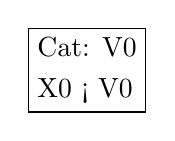
\begin{tikzpicture}[align=left]
%relative placement of nodes starting from the bottom: Future-CP
\node[draw](CPV0){Cat: V0  \\[1mm]
                  X0  <  V0};
\end{tikzpicture}
\zs
Das Zeichen `<' drückt aus, dass X0 unmittelbar vor V0 stehen muss. Goldberg argumentiert
für solche Konstruktionen, da die Kombination aus X0 und V0 nicht der Bedeutung der
Einzelteile entspricht.

Das Futur"=Hilfsverb\is{Verb!Hilfs-} \emph{x{\^a}stan} steht im Persischen immer direkt vor dem
Simplexverb, das in der Vergangenheitsform stehen muss. Goldberg drückt das wie folgt aus:
\eas
Futurhilfsverbkonstruktion nach \citew[\page 127]{Goldberg2003a}:\\
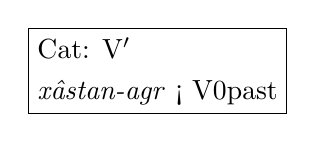
\begin{tikzpicture}[align=left]
\node[draw](Future){Cat: V$'$  \\[1mm]
                    \emph{x{\^a}stan-agr}  <  V0\sub{past}};
\end{tikzpicture}
\zs
Werden komplexe Prädikate ins Futur gesetzt, so steht das Futurhilfsverb zwischen dem X0
und dem V0 des komplexen Prädikats. Goldberg argumentiert, dass das Futurhilfsverb nicht als
Infix behandelt werden sollte, da es Kongruenzmerkmale trägt, die ja zur Flexionsmorphologie
zu zählen sind und da Flexion immer außerhalb von Derivation angewendet wird. Deshalb -- so argumentiert
sie -- liegt ein nicht direkt vorhersagbarer morphologischer Fakt vor, was die Stipulation einer
Futur"=Komplexes"=Prädikat"=Konstruktion rechtfertigt. 
% S. 16
Die Gemeinsamkeiten dieser Konstruktion
mit der Futurkonstruktion und der Komplexes"=Prädikat"=Konstruktion werden durch eine
entsprechende Vererbungshierarchie mit Defaultvererbung erfaßt, die in Abbildung~\vref{goldberg-persisch-vererbung}
dargestellt ist.
\begin{figure}
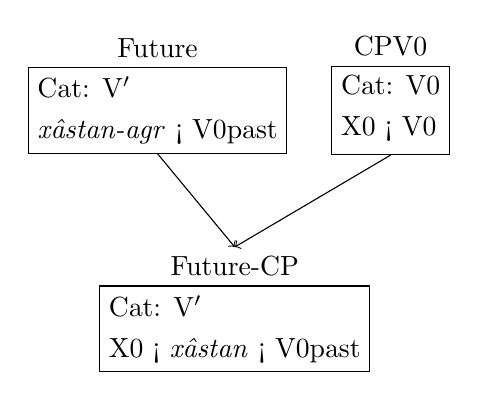
\begin{tikzpicture}[node distance=2.8cm,align=left]
%relative placement of nodes starting from the bottom: Future-CP

% Future-CP
\node[draw](Future-CP) at (0,0){Cat: V$'$  \\[1mm]
                                X0  < \emph{x{\^a}stan} <  V0\sub{past}};
\node[above] (Future-CP label) at (Future-CP.north) {Future-CP};

% Future
\node[draw,xshift=1cm](Future)[above left of=Future-CP label]{Cat: V$'$  \\[1mm]
                                             \emph{x{\^a}stan-agr}  <  V0\sub{past}};
\node[above] at (Future.north) {Future};

% CPV0
\node[draw](CPV0)[above right of=Future-CP label]{Cat: V0  \\[1mm]
                                            X0  <  V0\strut};
\node[above] at (CPV0.north) {CPV0};

\draw[->] (Future.south) to (Future-CP label.north);
\draw[->] (CPV0.south) to (Future-CP label.north);

\end{tikzpicture}
\caption{\label{goldberg-persisch-vererbung}%
Kombination der Komplexes"=Prädikat"=Konstruktion mit der Futurhilfsverbkonstruktion über Mehrfachvererbung mit Defaults}
\end{figure}
Wie man sieht, unterscheiden sich die beiden Konstruktionen, von denen die Futur"=Komplexes"=Prädikat"=Konstruktion
erbt: Sowohl die syntaktische Kategorie (V0 vs.\ V$'$)
als auch die lineare Abfolge der Konstruktionsbestandteile (\emph{x{\^a}stan-agr}  <  V0 vs.\ X0  <  V0)
sind verschieden. Diese Information wird bei der Unterkonstruktion, die von den beiden übergeordneten
Konstruktionen erbt, überschrieben.

\citet[\page 139--140]{Goldberg2003a} % S. 20
argumentiert dagegen, beim Vorliegen nicht"=transparenter Komplexes"=Verb"=Konstruktionen die Bedeutung
einem der Teile zuzuschreiben (also \emph{roSan} oder \emph{kardan} in (\mex{1})),
da die Bedeutung des komplexen Prädikats nur beim Vorliegen beider Bestandteile gegeben ist. 
\ea
\gll roSan kardan\\
     Licht tun\\\nopagebreak
\glt `einschalten'
\z
Das heißt aber, dass es zumindest für diese Fälle Unterkonstruktionen von CPV0 geben muss,
denn CPV0 beschreibt nur den allgemeinen Fall, Idiosynkratisches ist in diesem Muster noch nicht erfaßt.
Um zu erklären, was ein nicht"=transparentes komplexes Prädikat im Futur bedeutet, braucht man aber
eine Konstruktion, die vom nicht"=transparenten komplexen Prädikat und von der Futurkonstruktion erbt,
denn dieser Fall ist in Abbildung~\ref{goldberg-persisch-vererbung} noch nicht erfaßt. Das heißt,
dass es sowohl eine \emph{roSan kardan}"=Konstruktion als auch eine \emph{roSan x{\^a}stan kardan}"=Konstruktion
geben muss. Eine entsprechend modifizierte Hierarchie zeigt Abbildung~\vref{goldberg-persisch-vererbung-korrekt}.
\begin{figure}
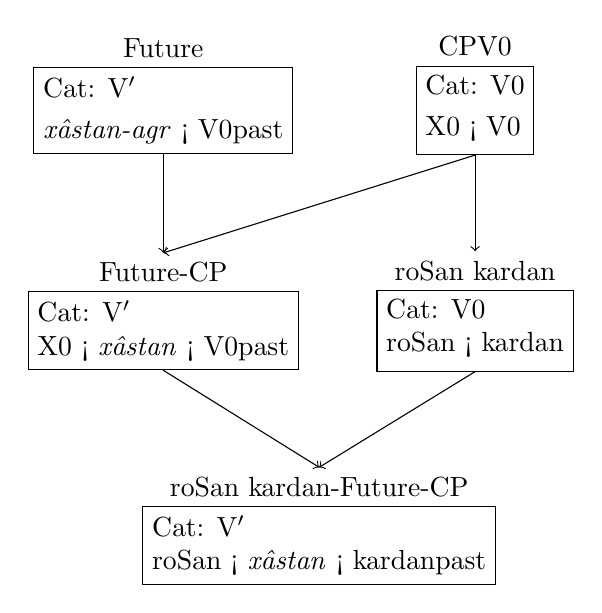
\begin{tikzpicture}[node distance=2.8cm,align=left]
%relative placement of nodes starting from the bottom: x0-xastan-V0
\node[draw](roSan kardan-Future-CP) at (0,0){Cat: V$'$  \\
                                roSan  < \emph{xâstan} <  kardan\sub{past}};
% Label
\node[above] (roSan kardan-Future-CP label) at (roSan kardan-Future-CP.north) {roSan kardan-Future-CP};

\node[draw](Future-CP)[above left of=roSan kardan-Future-CP label]{Cat: V$'$  \\
                                           X0  < \emph{xâstan}  <  V0\sub{past}};

% Label
\node[above] (Future-CP label) at (Future-CP.north) {Future-CP};

\node[draw](roSan kardan)[above right of=roSan kardan-Future-CP label]{Cat: V0  \\
                                            roSan  <  kardan\strut};

% Label
\node[above] (roSan kardan label) at (roSan kardan.north) {roSan kardan};

\node[draw](CPV0)[above of=roSan kardan]{Cat: V0  \\[1mm]
                                           X0  <  V0\strut};

\node[above] at (CPV0.north) {CPV0};

\node[draw](Future)[above of=Future-CP]{Cat: V$'$  \\[1mm]
                                 \emph{x{\^a}stan-agr}  <  V0\sub{past}};

\node[above] at (Future.north) {Future};


\draw[->] (Future-CP.south) to (roSan kardan-Future-CP label.north);
\draw[->] (roSan kardan.south) to (roSan kardan-Future-CP label.north);
\draw[->] (Future) to (Future-CP label);

\draw[->] (CPV0) to (roSan kardan label.north);
\draw[->] (CPV0.south) to (Future-CP label.north);
\end{tikzpicture}
\caption{\label{goldberg-persisch-vererbung-korrekt}%
Modifizierte Hierarchie nach Goldberg}
\end{figure}
Man muss also alle Kombinationen von nicht"=transparenten komplexen Prädikaten mit dem
Futurhilfsverb aufschreiben, was diesen Ansatz sehr unattraktiv macht. Man beachte, dass man sich
hier nicht dadurch aus der Affäre ziehen kann, dass man die Hierarchie, wie das von \citet{Koenig99a}
für Typhierarchien vorgeschlagen wurde, automatisch berechnen läßt, denn Goldbergs Spezifikationen
enthalten Defaults. \citet{Malouf2003a} schlägt zwar solch eine Berechnung auch für Typhierarchien
mit Defaultvererbung vor, schreibt aber, dass auf"|tretende Konflikte nach der Spezifität der 
Werte aufgelöst werden (\emph{while conflicts between default constraints are resolved according
to specificity} S.\,416). Für den Fall in Abbildung~\ref{goldberg-persisch-vererbung} (bzw.\
Abbildung~\ref{goldberg-persisch-vererbung-korrekt}) ist diese Strategie der Default"=Auflösung
nicht anwendbar, denn keine der beiden Beschränkungen \emph{x{\^a}stan-agr}  <  V0\sub{past}
und X0  <  V0 ist spezifischer als die andere. Das heißt, man kann die Berechnung der verschiedenen
Futur-CP"=Konstruktionen für nicht"=transparente komplexe Prädikate keinem automatischen Verfahren überlassen,
sondern muss alle Instanzen per Hand kodieren und die Werte, die die Unterkonstruktion nach Überschreibung
der Default"=Werte haben soll, für jede Konstruktion einzeln spezifizieren. Dass die Abfolge
von X0, Futur"=Hilfsverb und V0 für alle Fälle demselben Muster entspricht, wird in diesem
Ansatz nicht erfaßt, denn die entsprechende Information wird nicht ererbt, sondern für jede
einzelne Konstruktion neu spezifiziert.\footnote{
  Jochen Trommer\aimention{Jochen Trommer} (p.\,M.\ 2006) hat angemerkt, dass man diskontinuierliche
  Konstruktionen annehmen könnte. Die Boxen in Abbildung~\ref{goldberg-persisch-vererbung-korrekt}
  würden dann bedeuten, dass die Konstruktion \emph{x{\^a}stan-agr} und ein V0 dominiert bzw.\ ein X0
  und ein V0. Das `$<$' stünde\is{Linearisierung!-sdom"ane}\is{Linearisierung!-sregel} für Präzedenz
  statt für unmittelbare Präzedenz. Solche Linearisierungsbeschränkungen 
  würden bei der Vererbung keinen Konflikt erzeugen. (Sie könnten sogar unabhängig von den
  Konstruktionen angegeben werden, wie das in GPSG und HPSG gemacht wird.)

  Ähnliche Vorschläge für diskontinuierliche phrasale Konstruktionen wurden von \citet*[\page
  244--248]{Kathol95a} und \citet[Kapitel~4.2]{Crysmann2002a} für Partikelverben im Deutschen gemacht.
  Im Abschnitt~\ref{sec-disc-entry} wurden diese Analysen bereits verworfen.

  Das Problem, dass man Einbettung für die korrekte Erfassung der semantischen Eigenschaften der
  komplexen Prädikate braucht, besteht für Analysen mit diskontinuierlichen Prädikaten genauso wie
  für andere phrasale Analysen.
}

Darüber hinaus ergibt sich ein formales Problem, das auch im Kapitel~\ref{sec-vererbung-koenig} 
über Vererbung im Lexikon schon diskutiert wurde: Die Bedeutung des komplexen Prädikats wird unter
die Bedeutung des Futurhilfsverbs eingebettet. Das läßt sich aber per Vererbung nicht modellieren,
denn der Semantik"=Wert in der Unterkonstruktion überschreibt den Semantik"=Wert der von der
Komplexes"=Prädikat"=Konstruktion kommt \citep[Abschnitt~4.2]{MuellerPersian}. Dieses Problem läßt sich nur lösen, indem man Hilfsmerkmale
verwendet, wie das \citet[\page262]{Kathol94a} und \citet{Koenig99a} gemacht haben (siehe Kapitel~\ref{sec-vererbung-koenig}),
oder indem man verzeigerte Strukturen und Hilfsmerkmale zusammen mit Defaultvererbung verwendet 
\citep{MuellerDefaults}. In jedem Fall werden Hilfsmerkmale gebraucht, was die Theorie im Vergleich
zu Theorien, die ohne solche Merkmale auskommen, abwertet.
\is{Default|)}\il{Persisch|)}\is{Konstruktionsgrammatik (CxG)|)}

Betrachtet man die Daten genauer, stellt man fest, dass ähnliche Datenlagen aus dem Niederländischen
und aus deutschen Dialekten bekannt sind. So kann im Niederländischen\il{Niederländisch}
die Partikel aus Partikelverbkombinationen
durch Hilfsverben vom Verb getrennt werden:
\ea
\gll omdat Carol hem op kon  bellen\footnotemark\\
     weil  Carol ihn an kann rufen\\
\footnotetext{
\citew[\page126]{Koster75a}.
}
\glt `weil Carol ihn anrufen kann'
\z
Genauso muss im Thüringischen\is{Thüringisch} und im Fränkischen\is{Fränkisch} die Partikel vor den
Verben im Verbalkomplex stehen. \citet*[\page356]{Werner94a} gibt die folgenden Beispiele,
die nach Sperschneider\aimention{Heinz Sperschneider} zitiert sind
und im Nordwesten von Sonneberg/""Thüringen gesprochen wurden.
\eal
\label{ex-sonneberg-partikel-phasen}
\ex\iw{anfangen}
\gll a  \ldots{} hot aa   ze schimpfm  gfanga\\
     er {}       hat an   zu schimpfen gefangen\\
\glt `Er hat zu schimpfen angefangen.'
\ex\iw{aufhören}
\gll die  ham  \ldots{}  auf  zu arwettn ghört\\
     die haben {}        auf  zu arbeiten gehört\\
\glt `Die haben zu arbeiten aufgehört.'
\ex
\gll ham   sa  groud  aa mit assn  gfanga\\
     haben sie grade  an mit essen gefangen\\
\glt `Haben sie gerade zu essen angefangen?'
\zl

\noindent
Diese Daten kann man so analysieren, wie das in diesem Kapitel vorgeschlagen
wurde: Die Partikel wird vom Verb selegiert, die Gesamtbedeutung des Partikelverbs ist
beim Partikelverb spezifiziert. Wenn das Verb unter ein Futurhilfsverb eingebettet wird,
wird auch der Bedeutungsbeitrag des Partikelverbs unter die Futursemantik eingebettet.
Für Fälle wie in (\mex{0}) muss man annehmen, dass die Verbpartikel angehoben und
erst nach der Kombination von Hauptverb und Futurhilfsverb abgebunden wird \citep[\page29--30]{Mueller2005c}.


%\section*{Kontrollfragen}

\questions{
\begin{enumerate}
\item Ist \emph{umfahren} ein Partikelverb?
\end{enumerate}
}

%\section*{Übungsaufgaben}

\exercises{
\begin{enumerate}
\item Was braucht man für die Analyse der Sätze in (\mex{1})?
      \eal
      \ex Er kocht die Suppe vor.
      \ex Er arbeitet für Weihnachten vor.
      \zl
      Skizzieren Sie die syntaktischen Aspekte der Einträge für \emph{kochen} und für \emph{vor},
      und falls Sie der Meinung sind, dass keine der Lexikonregeln
      in diesem Kapitel anwendbar ist, geben Sie eine Lexikonregel
      an, die Partikelverben wie \emph{vorarbeiten}, \emph{vorkochen}
      und \emph{vorschlafen} zu ihren Basisverben in Beziehung setzt.

\item Laden Sie die zu diesem Kapitel gehörende Grammatik von der Grammix"=CD
(siehe Übung~\ref{uebung-grammix-kapitel4} auf Seite~\pageref{uebung-grammix-kapitel4}).
Im Fenster, in dem die Grammatik geladen wird, erscheint zum Schluß eine Liste von Beispielen.
Geben Sie diese Beispiele nach dem Prompt ein und wiederholen Sie die in diesem Kapitel besprochenen
Aspekte.

\end{enumerate}
}


\begin{comment}

Zurückgefallen sind das Saarland (von 7 auf 9) und Niedersachsen (von 8 auf 10)
jeweils um zwei Plätze. Jeweils um einen Platz zurück fielen Berlin (von 6 auf 7) und
Rheinland"=Pfalz (von 10 auf 11). c't 6/2005, S.\,102

\end{comment}


\furtherreading{
Partikelverben sind ein Thema, das die Linguisten immer wieder beschäftigt. Unter anderem wird
wieder und wieder diskutiert, ob Partikelverben in der Morphologie oder in der Syntax zu analysieren
sind. Die Anzahl der Publikationen zu Partikelverben im Deutschen und in anderen Sprachen ist
enorm. Hier sei nur auf die Monographie von Barbara \citet{Stiebels96a} und Andrew \citet{McIntyre2001a} und den Sammelband
\citew*{DJMU2002a-ed} verwiesen. Stiebels und McIntyre besprechen bestimmte Klassen von Partikelverben sehr genau.
Im Sammelband werden Partikelverben aus verschiedenen theoretischen Perspektiven beleuchtet.\is{Verb!Partikel-|)}

Die Diskussion der komplexen Prädikate im Persischen ist als \citew{MuellerPersian}
veröffentlicht. Die Diskussion phrasaler Analysen findet man in \citew{MuellerGTBuch1} und in \citew{MWArgSt}.
}